\documentclass{article}

\usepackage[T1]{fontenc}
\usepackage[utf8]{inputenc}
\usepackage{times}

\usepackage[font=small,labelfont=bf,tableposition=top]{caption}
\usepackage{graphicx}
\usepackage{natbib} 

\usepackage{amsmath}
\usepackage{amsfonts}
\usepackage{amssymb}
\usepackage{color, soul}
\usepackage{hyperref}
\usepackage{algorithmicx}
\usepackage{algpseudocode}
\usepackage{subfigure}
\usepackage{stmaryrd}

\renewcommand{\vec}[1]{\boldsymbol{{#1}}} 
\newcommand{\duesoon}[1]{{\sethlcolor{green}\hl{#1}}}
\usepackage{mathrsfs}


\newtheorem{theorem}{Theorem}
\newtheorem{acknowledgement}[theorem]{Acknowledgement}
\newtheorem{algorithm}[theorem]{Algorithm}
\newtheorem{axiom}[theorem]{Axiom}
\newtheorem{case}[theorem]{Case}
\newtheorem{claim}[theorem]{Claim}
\newtheorem{conclusion}[theorem]{Conclusion}
\newtheorem{condition}[theorem]{Condition}
\newtheorem{conjecture}[theorem]{Conjecture}
\newtheorem{corollary}[theorem]{Corollary}
\newtheorem{criterion}[theorem]{Criterion}
\newtheorem{definition}[theorem]{Definition}
\newtheorem{example}[theorem]{Example}
\newtheorem{exercise}[theorem]{Exercise}
\newtheorem{lemma}[theorem]{Lemma}
\newtheorem{notation}[theorem]{Notation}
\newtheorem{problem}[theorem]{Problem}
\newtheorem{proposition}[theorem]{Proposition}
\newtheorem{remark}[theorem]{Remark}
\newtheorem{solution}[theorem]{Solution}
\newtheorem{summary}[theorem]{Summary}
\newenvironment{proof}[1][Proof]{\textbf{#1.} }{\ \rule{0.5em}{0.5em}}

\newtheorem{guess}{Definition}
\newcommand{\comment}[1] {}
\newcommand{\Norder} {N}
\newcommand{\order}{\mathcal{O}}
\newcommand{\Npoints} {N_p}
\newcommand{\Nfaces} {N_{f}}
\newcommand{\Nelements} {N_e}

\newcommand{\eps}{\varepsilon}
\newcommand{\Dweak}{\wt{D}}
\newcommand{\diff}[2] {\frac{\partial #1}{\partial #2}}
\newcommand{\dxx}[2] {\frac{\partial^2 #1}{\partial {#2}^2}}
\newcommand{\difft}[2] {\frac{d #1}{d #2}}
\newcommand{\dxxt}[2] {\frac{d^2 #1}{d {#2}^2}}
\newcommand{\lagrange}[1] {\frac{d #1}{dt}}
\newcommand{\lebesgue}{\parallel I \parallel}
\newcommand{\polysp}{\mathcal{P}_N}
\newcommand{\laplacian}{\nabla^2}
\newcommand{\divergence}{\nabla \cdot}
\newcommand{\inte}{\int_{\mbox{\footnotesize ${\Omega_e}$}}}
\newcommand{\intb}{\int_{\mbox{\footnotesize ${\Gamma_e}$}}}
\newcommand{\intce}{\int_{\mbox{\footnotesize ${\widehat{\Omega}_e}$}}}
\newcommand{\intcb}{\int_{\mbox{\footnotesize ${\widehat{\Gamma}_e}$}}}
\newcommand{\intg}{\int_{\mbox{\footnotesize ${\Omega}$}}}
\newcommand{\intgb}{\int_{\mbox{\footnotesize ${\Gamma}$}}}
\newcommand{\intv}{\int_{\mbox{\footnotesize ${\sigma}$}}}
\newcommand{\sumv}{\sum_{K=1}^{N_{\mathrm{lev}}}}
\newcommand{\sumk}{\sum_{L=1}^{K}}
\newcommand{\sumN}{\sum_{i=1}^{N+1}}
\newcommand{\half}{\frac{1}{2}}
\newcommand{\inti}{\int_{\mbox{\footnotesize\sf I}}}
\newcommand{\intbd}{\oint_{\mbox{\footnotesize ${\delta}$\sf D}}}
\newcommand{\intbi}{\oint_{\mbox{\footnotesize ${\delta}$\sf I}}}
\newcommand{\ldnorm}[1]{\left\| #1 \right\|_{\mbox{\footnotesize \sf D}} }
\newcommand{\lonorm}[1]{\left\| #1 \right\|_{\Omega}}
\newcommand{\spc}[1]{\mbox{\sf #1}}
\newcommand{\ope}[1]{{\cal #1}}
\newcommand{\mt}[1]{{\rm #1}}
\newcommand{\dis}{\displaystyle}
\newcommand{\ve}{\varepsilon}
\newcommand{\ov}{\overline}
\newcommand{\wt}{\widetilde}
\newcommand{\wh}{\widehat}
\newcommand{\Dhat}{\widehat{D}}
\newcommand{\be}{\begin{equation}}
\newcommand{\ee}{\end{equation}}
\newcommand{\bea}{\begin{eqnarray*}}
\newcommand{\eea}{\end{eqnarray*}}
\newcommand{\Jace}{J^{(e)}}
\newcommand{\Jacl}{J^{(l)}}
\def\bepsilon{\mbox{\boldmath $\epsilon $}}
\def\bpsi{\mbox{\boldmath $\psi $}}
\def\bphi{\mbox{\boldmath $\phi $}}
\def\bmu{\mbox{\boldmath $\mu $}}
\def\Et{ \tilde{E} }
\def\Ht{ \tilde{H} }
\def\sdot{ \dot{\sigma} }

\newcommand{\fstar}{f^{(*)}}

\DeclareMathOperator{\Span}{span}
\DeclareMathOperator{\Dim}{dim}

\newcommand{\polyquad}{\mathcal{Q}_{N}}
\newcommand{\polyP}{\mathcal{P}_{N}}
\newcommand{\polyPnpm}{\mathcal{P}_{(N+M)}}
\newcommand{\polyPd}{\mathcal{P}_{d}}
\newcommand{\polyPnm}{\mathcal{P}_{N,M}}
\newcommand{\polyPn}{\mathcal{P}_{N,0}}
\newcommand{\transpose}{^{\mathcal{T}}}

\newcommand{\vecQ}{\vec{Q}}
\newcommand{\vecQe}{\vec{Q}^{(e)}}
\newcommand{\vecFe}{\vec{\mathcal{F}}^{(e)}}
\newcommand{\statevec}{\vec{Y}}
\newcommand{\statevecN}{\vec{Y}_N^{(e)}}
\newcommand{\statestage}{\vec{\mathcal{Y}}}
\newcommand{\Ftensor}{\vec{F}(\qvector)}
\newcommand{\FtensorN}{\vec{F}\left( \qvectorN \right)}
\newcommand{\FtensorStar}{\vec{F}\left( \qvector_N^{(e,k)} \right)}
\newcommand{\Svector}{S(\qvector)}
\newcommand{\SvectorN}{S \left( \qvectorN \right)}
\newcommand{\qref}{\vec{q}_0}
\newcommand{\qvectorb}{\vec{q}_b}
\newcommand{\qtt}{\vec{q}_{tt}}
\newcommand{\qhat}{\widehat{\vec{q}}}
\newcommand{\qhatb}{\widehat{\vec{q}}_b}
\newcommand{\qelem}{q^{(e)}}
\newcommand{\rhoref}{\rho_0}
\newcommand{\piref}{\pi_0}
\newcommand{\Thetaref}{\Theta_0}
\newcommand{\Gref}{G_0}
\newcommand{\Tref}{T_0}
\newcommand{\thetaref}{\theta_0}
\newcommand{\Pref}{{P}_0}
\newcommand{\Eref}{{E}_0}
\newcommand{\Href}{{h}_0}
\newcommand{\rhohat}{\widehat{\rho}}
\newcommand{\pihat}{\widehat{\pi}}
\newcommand{\Phat}{\widehat{P}}
\newcommand{\uvechat}{\widehat{{\mbox{\boldmath$u$\unboldmath}}}}
\newcommand{\uhathat}{\widehat{\widehat{{\mbox{\boldmath$u$\unboldmath}}}}}
\newcommand{\Uhat}{\widehat{{\mbox{\boldmath$U$\unboldmath}}}}
\newcommand{\Uhathat}{\widehat{\widehat{{\mbox{\boldmath$U$\unboldmath}}}}}
\newcommand{\thetahat}{\widehat{\theta}}
\newcommand{\Thetahat}{\widehat{\Theta}}
\newcommand{\Ehat}{\widehat{E}}
\newcommand{\uhat}{\widehat{u}}
\newcommand{\vhat}{\widehat{v}}
\newcommand{\what}{\widehat{w}}
\newcommand{\pitt}{\pi_{tt}}
\newcommand{\rhott}{\rho_{tt}}
\newcommand{\Ett}{E_{tt}}
\newcommand{\Utt}{\vec{U}_{tt}}
\newcommand{\uvectt}{\vec{u}_{tt}}
\newcommand{\utt}{u_{tt}}
\newcommand{\vtt}{v_{tt}}
\newcommand{\wtt}{w_{tt}}
\newcommand{\Ptt}{P_{tt}}
\newcommand{\vecPtt}{\vec{P}_{tt}}
\newcommand{\Thetatt}{\Theta_{tt}}
\newcommand{\thetatt}{\theta_{tt}}
%Projector Matrices
\newcommand{\projmatrix}{\vec{\mathcal{P}}}
\newcommand{\qmatrix}{\vec{\mathcal{Q}}}
\newcommand{\pcmatrix}{\vec{\mathcal{P}}_C}
\newcommand{\Cmatrix}{\left(\vec{\mathcal{C}}^{(e,f)}\right)\transpose}
\newcommand{\Dmatrix}{\vec{D}^{(e)}}
\newcommand{\Dwmatrix}{\wt{\vec{D}}^{(e)}}
\newcommand{\Mmatrix}{M^{(e)}}
\newcommand{\Fmatrix}{\vec{F}^{(e,l)}}
\newcommand{\Gmatrix}{\mathcal{G}}
\newcommand{\Umatrix}{\mathcal{U}^{(e,f)}}
\newcommand{\amatrix}{\vec{\mathcal{A}}}
\newcommand{\rmatrix}{\vec{\mathcal{R}}}
%Vectors
\newcommand{\nvector}{\wh{\vec{n}}_{\Gamma}}
\newcommand{\nhat}{\wh{\vec{n}}}
\newcommand{\ivector}{\wh{\vec{i}}}
\newcommand{\jvector}{\wh{\vec{j}}}
\newcommand{\kvector}{\wh{\vec{k}}}
\newcommand{\rvector}{\wh{\vec{r}}}
\newcommand{\svector}{\wh{\vec{s}}}
\newcommand{\tvector}{\wh{\vec{t}}}
\newcommand{\vvector}{\wh{\vec{v}}}
\newcommand{\Qvector}{\vec{Q}}
%Vectors
\newcommand{\ur}{{u}^{(r)}}
\newcommand{\us}{{u}^{(s)}}
\newcommand{\ut}{{u}^{(t)}}
\newcommand{\urtt}{{u}_{tt}^{(r)}}
\newcommand{\ustt}{{u}_{tt}^{(s)}}
\newcommand{\uttt}{{u}_{tt}^{(t)}}
\newcommand{\urhat}{\widehat{u}^{(r)}}
\newcommand{\ushat}{\widehat{u}^{(s)}}
\newcommand{\uthat}{\widehat{u}^{(t)}}
%Other Operators
\newcommand{\grad}{\vec{\nabla}}
\newcommand{\Grad}{\vec{\nabla}}
\newcommand{\Dskew}{\mathcal{D}}

\def\bepsilon{\mbox{\boldmath $\epsilon $}}
\def\bpsi{\mbox{\boldmath $\psi $}}
\def\bphi{\mbox{\boldmath $\phi $}}
\def\bmu{\mbox{\boldmath $\mu $}}
\def\Et{ \tilde{E} }
\def\Ht{ \tilde{H} }
\def\sdot{ \dot{\sigma} }
%\renewcommand{\thetable}{\Roman{table}}
%\renewcommand{\thefigure}{\arabic{figure}}

%\DeclareMathOperator{\Span}{span}
%\DeclareMathOperator{\Dim}{dim}

%Editing Commands
\newcommand{\here}{ \textcolor{red}{YOU ARE HERE}}

%Time-Integration
\newcommand{\dt}{{\Delta t}}
\newcommand\ST{\rule[-0.75em]{0pt}{2em}}
\newcommand{\Sfunction}{\mathcal{S}}
\newcommand{\Lfunction}{\mathcal{L}}
\newcommand{\Nfunction}{\mathcal{N}}

%DG Operators
\newcommand{\average}[1]{ \left\{ #1 \right\} }
\newcommand{\jump}[1]{ \llbracket #1 \rrbracket }

%HDG Matrices
\newcommand{\CCmatrix}{\mathcal{C}^{(e,k)}}
\newcommand{\Jmatrix}{\mathcal{J}^{(e,k)}}
\newcommand{\DDmatrix}{\wt{D}^{(e)}}
\newcommand{\SSvector}{\mathcal{S}(q)}
\newcommand{\cghdg}{cg\underline{\hspace{0.15cm}}to\underline{\hspace{0.15cm}}hdg}
%\newcommand{\ul}{\underline{\hspace{0.15cm}}}
\newcommand{\RRmatrix}{\mathcal{R}}

%Clima specific variables
\newcommand{\etotal}{e^{\mathrm{tot}}}
\newcommand{\Etotal}{E^{\mathrm{tot}}}
\newcommand{\Fvector}{\vec{\mathcal{F}}}
\newcommand{\Pvector}{\vec{\mathcal{P}}}
\newcommand{\Fadv}{\vec{\mathcal{F}}^{\mathrm{adv}}}
\newcommand{\Fndf}{\vec{\mathcal{F}}^{\mathrm{ndf}}}
\newcommand{\Fdiff}{\vec{\mathcal{F}}^{\mathrm{diff}}}
\newcommand{\Tvector}{\vec{\mathcal{T}}}
\newcommand{\Source}{\vec{\mathcal{S}}}

\newcommand{\fxg}[1]{\textcolor{cyan}{FXG: #1}}



\title{Design Document for the CLIMA Atmosphere Model} 
\author{ }

\begin{document}

\maketitle
\tableofcontents

\section{Introduction}
\label{sec:introduction}

This document highlights the design specifications for the atmosphere model that is part of the Climate Machine (CLIMA). We refer to this atmosphere model as CLIMA-atmos. The model is designed to run both in a global configuration and in a large-eddy simulation (LES) configuration from the same code base.  

\section{Thermodynamics of Moist Air}\label{s:thermodynamics}

The thermodynamics of moist air is often subject to empirical approximations, which usually are opaque, internally inconsistent, and/or inconsistent across model components. For example, microphysical process models often use different approximations for thermodynamic quantities such as saturation vapor pressures than the dynamical core. The often bewildering array of approximations makes it difficult to achieve global conservation, e.g., of energy, and it complicates the use of models for other planetary atmospheres, with different thermodynamic parameters. 

Here we employ one consistent set of thermodynamic approximations for all model components. These result in straightforward, easily adaptable, and relatively accurate expressions for thermodynamic quantities, including closed-form expressions of saturation vapor pressures in terms of thermodynamic parameters. The key to thermodynamic consistency at reasonable accuracy is to take the specific heat capacities of the constituents of moist air (dry air, water vapor, liquid water, and ice) to be constant. All other thermodynamic quantities can then be derived \citep[cf.][]{Romps08a,Marquet16a}. 

\subsection{Working Fluid and Equation of State}

The working fluid of the atmosphere model is moist, potentially cloudy air, considered to be an ideal mixture of dry air, water vapor, and condensed water (liquid and ice) suspended in clouds. Dry air and water vapor are taken to be ideal gases. The specific volume of the cloud condensate is neglected relative to that of the gas phases (it is a  factor $10^{3}$ less than that of the gas phases). All phases are assumed to have the same temperature and move with the working fluid. However, although the suspended cloud condensates are moving with the fluid, they need not be in thermodynamic equilibrium with the other fluid constituents; out-of-equilibrium phases such as supercooled liquid can exist. Falling condensate (precipitation) is not considered part of the working fluid and is treated separately.

The density of the moist air is denoted by $\rho$. We use the following notation for the mass fractions of the moist air mixture (mass of a constituent divided by the total mass of the working fluid):
\begin{itemize}
\item $q_d$: dry air mass fraction,
\item $q_v$: water vapor specific humidity,
\item $q_l$: liquid water specific humidity,
\item $q_i$: ice specific humidity,
\item $q_c = q_l + q_i$: condensate specific humidity,
\item $q_t = q_v + q_c$: total specific humidity.
\end{itemize}
Because this enumerates all constituents of the working fluid, we have $q_t + q_d = 1$. In Earth's atmosphere, the water vapor specific humidity $q_v$ generally dominates the total specific humidity $q_t$ and is usually $\order(10^{-2})$ or smaller; the condensate specific humidity is typically $\order(10^{-4})$. Hence, water is a trace constituent of the atmosphere, and only a small fraction of atmospheric water is in condensed phases. 

The pressure $p$ of the working fluid is the sum of the partial pressures of dry air and water vapor, both taken to be ideal gases. Neglecting the volume of the condensed phases (but not their masses), this gives $p = \rho (R_d q_d + R_v q_v) T$, where $R_d$ is the specific gas constant of dry air, and $R_v$ is the specific gas constant of water vapor. Since $q_d = 1-q_t$ and $q_v = q_t - q_c$, this can also be written as
\begin{equation}
    p = \rho R_m T,
\label{eq:eos}
\end{equation}
where
\begin{equation}
    R_m = R_d \left[1 + (\eps_{dv}-1)q_t - \eps_{dv} q_c\right]
\label{eq:R_m}
\end{equation}
is the specific gas ``constant'' of moist air (which is not a constant), and $\eps_{dv} = R_v/R_d$ is the ratio of the molar masses of dry air and water vapor ($\eps_{dv} \approx 1.61$). Equations~\eqref{eq:eos} and \eqref{eq:R_m} constitute the equation of state of the working fluid.

\subsection{Heat Capacities}\label{s:heat_capacities}

The isochoric specific heat capacities of the constituents of moist air are:
\begin{enumerate}
    \item $c_{vd}$: Isochoric specific heat capacity of dry air;
    \item $c_{vv}$: Isochoric specific heat capacity of water vapor;
    \item $c_{vl}$: Isochoric specific heat capacity of liquid water;
    \item $c_{vi}$: Isochoric specific heat capacity of ice.
\end{enumerate}
Our key thermodynamic approximation is to take these isochoric specific heat capacities to be constants. This is an approximation because they depend weakly on temperature. But for atmospheric conditions, the error of approximating them as constant is less than 1\% for dry air, the main constituent of moist air, and at most a few percent for the water phases.

The difference between the isochoric and isobaric specific heat capacities is proportional to the specific volume. Consistent with taking the specific volume of liquid water and ice to be zero, we take the isochoric and isobaric specific heat capacities of the condensed phases to be equal. The isobaric specific heat capacities of the constituents then are:
\begin{enumerate}
    \item $c_{pd} = c_{vd} + R_d$: Isobaric specific heat capacity of dry air;
    \item $c_{pv} = c_{vv} + R_v$: Isobaric specific heat capacity of water vapor;
    \item $c_{pl} = c_{vl}$: Isobaric specific heat capacity of liquid water;
    \item $c_{pi} = c_{vi}$: Isobaric specific heat capacity of ice.
\end{enumerate}

The corresponding specific heat capacities of moist air are the weighted sum of those of the constituents:
\begin{align}
    c_{\cdot m} & = (1-q_t) c_{\cdot d} + q_v c_{\cdot v} + q_l c_{\cdot l} + q_i c_{\cdot i}\\
    & = c_{\cdot d} + (c_{\cdot v} - c_{\cdot d})q_t + (c_{\cdot l} - c_{\cdot v})q_l + (c_{\cdot i} - c_{\cdot v})q_i
\end{align}
where $\cdot$ stands for $v$ or $p$ and we have used $q_v = q_t -q_l - q_i$.

\subsection{Latent Heats}

Kirchoff's relation states that the specific latent enthalpy (heat) $L$ of a phase change depends on temperature $T$ through
\begin{equation}
    \frac{dL}{dT} = \Delta c_p,
\end{equation}
where $\Delta c_p$ is the difference in isobaric specific heat capacities between the phase with the higher specific volume and that with the lower specific volume. For the constant isobaric specific heat capacities that we assume, this can be integrated to give
\begin{equation}
    L = L_0 + \Delta c_p (T-T_0),
    \label{eq:LH_temperature}
\end{equation}
where $T_0$ is a reference temperature and $L_0$ is the latent heat at $T_0$. 

For the phase transitions of water, this implies specifically:
\begin{enumerate}
    \item $L_v = L_{v,0} + (c_{pv} - c_{pl}) (T - T_0)$: Latent heat of vaporization;
    \item $L_f = L_{f,0} + (c_{pl} - c_{pi}) (T - T_0)$: Latent heat of fusion;
    \item $L_s = L_{s,0} + (c_{pv} - c_{pi}) (T - T_0)$: Latent heat of sublimation.
\end{enumerate}

\subsection{Internal Energies}\label{s:internal_energies}

The specific internal energies of the constituents of moist air can be written as
\begin{subequations}\label{e:internal_energies}
\begin{align}
I_d(T) & = c_{vd} (T - T_0),  \\
I_v(T) & = c_{vv} (T - T_0) + I_{v,0},\\
I_l(T) & = c_{vl} (T - T_0), \\
I_i(T) & = c_{vi} (T - T_0) - I_{i,0}.
\end{align}
\end{subequations}
Here, the reference specific internal energy $I_{v,0}$ is the difference in specific internal energy between vapor and liquid at the reference temperature $T_0$, and $I_{i,0}$ is the difference in specific internal energy between ice and liquid at $T_0$. The internal energy of moist air is the weighted sum of that of the constituents,
\begin{equation}
\begin{split}
     I(T) & = (1-q_t) I_d(T) + q_v I_v(T) + q_l I_l(T) + q_i I_l(T)\\
          & = c_{vm} (T - T_0)  + q_v I_{v,0} - q_i I_{i,0}.
     \label{eq:total_internal_energy}
\end{split}
\end{equation}
The internal energy can be inverted to obtain the temperature given $I$ and the specific humidities,
\begin{equation}
    T = T_0 + \frac{I - (q_t - q_l) I_{v,0} + q_i (I_{i,0} + I_{v,0})}{c_{vm}},
    \label{eq:temperature}
\end{equation}
where we have used $q_v = q_t - q_l - q_i$. This allows one to recover temperature given internal energy and specific humidities as state variables.

The reference specific internal energies $I_{v,0}$ and $I_{i,0}$ are related to the reference specific latent heats $L_{v,0}$ and $L_{f,0}$, which indicate the enthalpy differences between the phases at $T_0$. The reference specific internal energies are obtained from the reference specific latent heats by subtracting the ``$pV$'' term, which is $p_k/\rho_k$ for the relevant partial pressure $p_k$ and specific volume $1/\rho_k$ of the phase $k$. This gives
\begin{subequations}\label{e:ref_internal_energies}
\begin{align}
     I_{v,0} &= L_{v, 0} - R_v T_0,\\
     I_{i,0} &= L_{f, 0},
\end{align}
\end{subequations}
where we again neglected the specific volume of the condensed phases. 
   
\subsection{Enthalpies}\label{s:enthalpies}

The specific enthalpies of the constituents of moist air are obtained by adding $p_k/\rho_k$ for phase $k$ to the corresponding specific internal energy \eqref{e:internal_energies}. Again neglecting the specific volumes of the condensed phases and using the relations \eqref{e:ref_internal_energies} between reference specific energies and latent heats, and the relations between isochoric and isobaric heat capacities, this gives:
\begin{subequations}
\begin{align}
    h_d(T) = I_d(T) + R_d T &= c_{pd}(T-T_0) + R_d T_0, \\
    h_v(T) = I_v(T) + R_v T &= c_{pv}(T-T_0) + L_{v,0}, \\
    h_l(T) = I_l(T) \hphantom{{\,}+ R_d T} &= c_{pl}(T-T_0), \\
    h_i(T) = I_i(T) \hphantom{{\,}+ R_d T} &= c_{pi}(T-T_0) - L_{f,0}.
\end{align}
\end{subequations}
The enthalpy of moist air is the weighted sum of the constituent enthalpies:
\begin{equation}
\begin{split}
    h   &= (1-q_t) h_d + q_v h_v + q_l h_l + q_i h_i \\
        &= c_{pm} (T-T_0) + q_v L_{v,0} - q_i L_{i,0} + (1-q_t) R_d T_0\\
        &= I(T) + R_m T.
\end{split}
\end{equation}

The enthalpy is the relevant thermodynamic energy quantity in fluid transport. It arises in boundary conditions for energy fluxes and in the modeling of SGS turbulent transport. For those purposes, we need gradients of the enthalpy, which can be written as 
\begin{equation}\label{e:enthalpy_gradient}
    \nabla h = c_{pm} \nabla T - h_d \nabla q_t
    + h_v(T) \nabla q_v + h_l(T) \nabla q_l + h_i(T) \nabla q_i.
\end{equation}
This cleanly separates gradients involving temperature and gradients involving specific humidities.

\subsection{Saturation Vapor Pressure}

The Clausius-Clapeyron relation describes how the saturation vapor pressure $p_v^*$ of an ideal gas over a plane surface of condensate depends on temperature:
\begin{equation}
    \frac{d \log(p_v^*)}{dT} = \frac{L}{R_v T^2}.
\end{equation}
Here, $L$ is the latent heat of the phase transition, which may be $L_v$ for the saturation vapor pressure over liquid, or $L_s$ for the saturation vapor pressure over ice. Substituting the linear relation \eqref{eq:LH_temperature} between latent heat and temperature, and taking $p_\mathrm{tr}$ to be the vapor pressure at the triple point (by definition equal to the saturation vapor pressures both over liquid and ice), the Clausius-Clapeyron relation can be integrated to give a closed-form expression for the vapor pressure that is consistent with our thermodynamic assumptions:
\begin{equation}
    p_v^* = p_{\mathrm{tr}} \left( \frac{T}{T_{\mathrm{tr}}} \right)^{\frac{\Delta c_p}{R_v}}
        \exp \left[ \frac{L_0 - \Delta c_p T_0}{R_v} 
        \left( \frac{1}{T_{\mathrm{tr}}} - \frac{1}{T} \right) \right].
        \label{eq:sat_vapor_pressure}
\end{equation}
With $L_0 = L_{v,0}$ or $L_0 = L_{s,0}$ and the corresponding heat capacity difference $\Delta c_p$, this gives saturation vapor pressures over liquid or ice that are accurate within 3\% for temperatures between 200 and 330~K (with accuracy better than 1\% for typical near-surface conditions).

To obtain the saturation vapor pressure over a mixture of liquid and ice (e.g., in mixed-phase clouds), using a weighted average of the relevant specific latent heats in the vapor pressure \eqref{eq:sat_vapor_pressure} leads to a thermodynamically consistent formulation \citep{Pressel15a}. That is, if a fraction $\lambda$ of the condensate is liquid and the complement $1-\lambda$ is ice, calculating the saturation vapor pressure with a latent heat $\lambda L_v + (1-\lambda)L_s$ gives a thermodynamically consistent saturation vapor pressure over the mixture. In thermodynamic equilibrium, the liquid fraction $\lambda(T) = \mathcal{H}(T-T_{\mathrm{freeze}})$ is a Heaviside function $\mathcal{H}$ of temperature, being zero 0 below the freezing temperature $T_{\mathrm{freeze}}$ and 1 above it. However, out of thermodynamic equilibrium, supercooled liquid can exist between the temperature of homogeneous ice nucleation and the freezing temperature.

\subsection{Saturation Specific Humidity}
\label{sct:sat_spef_hum}
From the saturation vapor pressure $p_v^*$, the saturation specific humidity can be computed using the ideal gas law \eqref{eq:eos}, giving the density of water vapor at saturation $\rho_v^* = p_v^*(T)/(R_v T)$, and hence the saturation specific humidity 
\begin{equation}\label{eq:sat_shum}
     q_v^* = \frac{\rho_v^*}{\rho} = \frac{p_v^*(T)}{\rho R_v T}.
\end{equation}

\subsection{Saturation Adjustment}
\label{sct:sat_adj}
Gibbs' phase rule states that in thermodynamic equilibrium, the temperature $T$ and liquid and ice specific humidities $q_l$ and $q_i$ can be obtained from the three thermodynamic state variables density $\rho$, total water specific humidity $q_t$, and internal energy $I$. Thus, a moist dynamical core that assumes equilibrium thermodynamics can be obtained from a dry dynamical core with total energy as a prognostic variable by including only a tracer for the total specific humidity $q_t$, and calculating the temperature and condensate specific humidities from $\rho$, $q_t$, and $I$. 

Because the temperature \eqref{eq:temperature} depends on the condensate specific humidities at saturation (equilibrium), which in turn depend nonlinearly on temperature, obtaining the temperature and condensate specific humidities from the state variables $\rho$, $q_t$, and $I$ is a nonlinear problem. It is the problem of finding the root $T$ of
\begin{equation}\label{e:sat_adjustment}
I - I^*(T; \rho, q_t) = 0,
\end{equation}
where $I^*(T; \rho, q_t)$ is the internal energy at saturation, with $q_v = q_v^*(T, \rho)$ and with the saturation excess (total condensate) $q_c = \max(q_t - q_v^*, 0)$ partitioned according to the liquid fraction $\lambda(T)$ into liquid $q_l = \lambda q_c$ and ice $(1-\lambda)q_c$. This nonlinear problem must be solved iteratively or approximately, in what is known as a saturation adjustment procedure. 

Using saturation adjustment makes it possibly to construct a moist dynamical core that has the total specific humidity $q_t$ as the only prognostic moisture variable. The price for this simplicity is the necessity to solve a nonlinear problem iteratively (or approximately) at each time step, and being confined to an equilibrium thermodynamics framework. Using explicit tracers for the condensates $q_l$ and $q_i$ in addition to $q_t$ avoids iterations at each time step and allows the inclusion of explicit non-equilibrium processes, such as those leading to the formation of supercooled liquid in mixed-phase clouds. 

\subsection{Auxiliary Thermodynamic Functions}

Several auxiliary thermodynamic functions are commonly used. 

\paragraph{Potential temperature.} The potential temperature $\theta$ is the temperature an air mass would have if brought adiabatically from pressure $p$ and temperature $T$ to some reference pressure $p_0$ (typically taken to be mean sea level pressure):
\begin{equation}\label{e:pot_temp_press_T}
\theta = T \left( \frac{p_0}{p} \right)^\kappa \quad \text{with} \quad \kappa = \frac{R_m}{c_{pm}}.
\end{equation}
Note that the adiabatic exponent $\kappa$ takes the effect of  moisture on the effective gas ``constant'' and specific heat capacity of air into account.

\paragraph{Virtual (potential) temperature.} The virtual or density temperature $T_v$ is the temperature dry air would need to have to have the same density as moist air at the same pressure. Using the ideal gas law $p/\rho = R_m T$, this implies $R_m T  = R_d T_v $, or
\begin{equation}\label{e:virtual_temp}
T_v = \frac{R_m}{R_d} T.
\end{equation}

A virtual potential temperature can be defined analogously:
\begin{equation}\label{e:virtual_pottemp}
\theta_v = \frac{R_m}{R_d} \theta.
\end{equation}
Some texts distinguish virtual and density (potential) temperatures, where density (potential) temperatures take the mass of condensate into account, whereas virtual (potential) temperatures do not. We always take the mass of any condensate into account in the thermodynamics of moist air and do not make that distinction here. 

\paragraph{Speed of sound.} The speed of sound in (moist) air is 
\begin{equation}\label{e:soundspeed}
 c_s = (\gamma R_m T)^{1/2}, \qquad \gamma = \frac{c_{pm}}{c_{vm}},
\end{equation}
with the appropriate gas constants for moist air.

\section{Governing Equations}
\label{sec:governing_equations}

\subsection{Mass Balance}

Moist air mass satisfies the conservation equation
\begin{equation}
\diff{\rho}{t} + \divergence (\rho\vec{u}) = \rho \mathcal{S}_{q_t},
\label{eq:governing_equations/mass}
\end{equation}
where $\vec{u}$ is the three-dimensional advective velocity vector, understood to be the velocity of the barycenter of the moist air elements. Moist air mass is not exactly conserved where precipitation forms, sublimates, or evaporates, or where water diffuses \citep{Bott08a}. The  right-hand side involves the local source/sink of water mass $\mathcal{S}_{q_t}$ owing to precipitation formation, evaporation/sublimation of precipitating hydrometeors (generally provided by a microphysics parameterization), or diffusion of water. 

The water mass sources/sinks usually are about two orders of magnitude smaller than the other terms in the mass balance. However, there is evidence that their effect is important, e.g., in strongly precipitating tropical cyclones \citep{Qiu93a,Lackmann04a}. They are zeroth-order important in some other planetary atmospheres, in which the condensable species is a major constituent of the atmosphere. For example, CO\textsubscript{2} is the primary constituent of Mars' atmosphere and seasonally condenses onto the winter pole, leading to large effects of mass non-conservation on the flow \cite[e.g.,][]{Soto15a}. Since we want to be able to use CLIMA-atmos for other planetary atmospheres, we are taking such mass sources/sinks into account.

\subsection{Moisture Balances}

Total water satisfies the conservation equation
\begin{equation}
\diff{(\rho q_t)}{t} + \divergence (\rho q_t \vec{u}) = \rho \mathcal{S}_{q_t}.   
\label{eq:governing_equations/moisture}
\end{equation}
The right-hand side is the same as that in the conservation law \eqref{eq:governing_equations/mass} for total mass, which means that the dry air mass $(1-q_t)\rho$ is exactly conserved, and deviations from conservation of the moist air mass $\rho = (1-q_t)\rho + q_t \rho$ arise from deviations from conservation of total water $q_t\rho$. The conservation laws for mass \eqref{eq:governing_equations/mass} and total water \eqref{eq:governing_equations/moisture} together imply the material derivative 
\[
\frac{dq_t}{dt} = (1-q_t) \mathcal{S}_{q_t},
\]
with the factor $(1-q_t)$ arising because both the density of moist air $\rho$ and the density of water $\rho_t$ enter $q_t = \rho_t/\rho$, and both change simultaneously when $\mathcal{S}_{q_t}$ is nonzero.

The sources/sink of total water can be written as  
\begin{equation}\label{e:water_sources}
     \rho \mathcal{S}_{q_t} = - \rho C(q_t \rightarrow q_p) - \divergence (\rho \vec{d}_{q_t}),
\end{equation}
with evaporation or sublimation of precipitation and formation of precipitation contributing to the conversion from $q_t$ to $q_p$ (i.e., $C(q_t \rightarrow q_p)$), and diffusive and SGS turbulent fluxes of moisture captured by $\vec{d}_{q_t}$. The diffusive or SGS turbulent flux of water consists of fluxes of water vapor, cloud liquid, and cloud ice, \begin{equation}
    \vec{d}_{q_t} =\vec{d}_{q_v} + \vec{d}_{q_l} + \vec{d}_{q_i},
\end{equation}
where $q_v = q_t - q_l - q_i$.

If the suspended condensates (cloud liquid and ice) are in local thermodynamic equilibrium with the gas phase, Gibbs' phase rule implies that their specific humidities, $q_l$ and $q_i$, can be determined by saturation adjustment \eqref{e:sat_adjustment} from three other thermodynamic state variables, such as density $\rho$, total water specific humidity $q_t$, and internal energy $I$. However, to enable the explicit modeling of out-of-equilibrium phases (e.g., supersaturated water vapor in the upper troposphere or supercooled liquid water in mixed-phase clouds), we explicitly model the specific humidities of suspended liquid ($q_l$) and ice ($q_i)$. They satisfy conservation equations of the form
\begin{equation}
\diff{(\rho q_k)}{t} + \divergence (\rho q_k \vec{u}) = \rho \mathcal{S}_k  -\divergence (\rho \vec{d}_ci
{q
_k}),   
\label{eq:governing_equations/condensate}
\end{equation}
where $k \in \{l, i\}$ indicates the phase and 
\begin{align}
    \mathcal{S}_l & = C(q_i \rightarrow q_l) + C(q_v \rightarrow q_l) + C(q_p \rightarrow q_l), \\
    \mathcal{S}_i & = C(q_l \rightarrow q_i) + C(q_v \rightarrow q_i) + C(q_p \rightarrow q_i)
\end{align}
represent sources of cloud liquid and ice. The terms $C(q_j \rightarrow q_{l/i}) = - C(q_{l/i} \rightarrow q_j)$ represent the conversion of species $j \in \{l, i, v, p\}$ to cloud liquid $q_l$ or cloud ice $q_i$, with $q_p$ representing the mass fraction of precipitation. The conversion terms include processes such as evaporation or sublimation of cloud condensate, melting of cloud ice, or precipitation formation, all provided by microphysics parameterizations. The conversion term $C(q_t \rightarrow q_p) = -C(q_p \rightarrow q_t)$ in equation \eqref{e:water_sources} for total water is the sum of the conversion terms
\begin{equation}
    C(q_t \rightarrow q_p) = C(q_v \rightarrow q_p) + C(q_l \rightarrow q_p) + C(q_i \rightarrow q_p)
\end{equation}
from vapor, liquid, and ice to precipitation. 

\subsection{Momentum Balance}

The vector invariant form of the momentum equation in a coordinate system rotating with constant angular velocity $\vec{\Omega}$ is 
\begin{equation}
\diff{(\rho\vec{u})}{t} + \divergence \left( \rho\vec{u} \otimes \vec{u} + p \vec{I}_3\right) =  - \rho \grad\Phi - 2\vec{\Omega} \times \rho\vec{u} - \divergence (\rho \vec{\tau}) - \divergence\left( \vec{d}_{q_t} \otimes \rho\vec{u} \right) + \rho \vec{F}_u
\label{eq:governing_equations/momentum}
\end{equation}
where $\vec{I}_3$ is the rank-3 identity matrix; $\Phi$ is the effective gravitational potential (including centrifugal accelerations); $\vec{\tau}$ is a viscous and/or SGS momentum flux tensor (negative of viscous or SGS stress tensor); and $\vec{F}_u$ is any other body force that may be applied (e.g., a drag force). The tensor involving the diffusive flux of water, $\vec{d}_{q_t} \otimes \rho\vec{u}$, represents the momentum flux carried by water that is diffusing (it is usually very small). Mechanical interactions between falling precipitation and the fluid, giving rise to frictional drag on the fluid in shear zones around falling hydrometeors \citep{Pauluis00}, are taken to be included in the momentum flux tensor $\vec{\tau}$. Momentum and kinetic energy transport by precipitating hydrometeors is neglected; it is 3--4 orders of magnitude smaller than other terms in the budgets \citep{Romps08a}.

These are the general, deep-atmosphere equations for a moist, nonhydrostatic atmosphere, without the thin-shell approximation traditionally made in climate models. (The thin-shell approximation assumes that in the formulation of the angular momentum, the distance from any point in the atmosphere to the barycenter of the planet is a constant and equal to the mean planetary radius.)

\subsection{Energy Balance}

To close the equations of motion for the working fluid, we require a thermodynamic or energy balance equation. Various choices are possible, a temperature (internal energy or enthalpy) equation being most common in climate models. We instead use the total specific energy $e^\mathrm{tot}$ to close the system, as in \citet{Romps08a}, a quantity that is conserved in reversible moist processes such as phase transitions of water. 

Total energy satisfies the conservation law \citep{Romps08a,Bott08a} 
\begin{multline}
 \diff{(\rho e^\mathrm{tot})}{t} + \divergence \left( (\rho e^\mathrm{tot} + p)\vec{u} \right)
 = -\divergence (\rho \vec{F}_R) - \divergence (\rho \vec{J}) + \rho Q - \divergence (\rho \vec{D})  \\
  - \divergence (\vec{u} \cdot \rho\vec{\tau)} + \rho \vec{u} \cdot \vec{F}_u \\
   - \sum_{j\in\{v,l,i\}}(I_j + \Phi)  \rho C(q_j \rightarrow q_p) - M,
 \label{eq:energy_balance}
\end{multline}
where the total specific energy $e^{\mathrm{tot}}$ is the weighted sum of the total specific energies of the moist air constituents (dry air, water vapor, cloud liquid, cloud ice):
\begin{equation}\label{e:energy_sum}
    e^{\mathrm{tot}} = (1-q_t) e_d^{\mathrm{tot}} + q_v e_v^{\mathrm{tot}} + q_l e_l^{\mathrm{tot}} + q_i e_i^{\mathrm{tot}}.
\end{equation}
Each constituent is assumed to be moving with the same velocity and to have the same temperature, so that the constituent specific energies can be written as
\begin{subequations}\label{e:constituent_energies}
\begin{align}
e_d^{\mathrm{tot}} & = \frac{1}{2} \| \vec{u} \|^2 + \Phi + I_d(T), \\
e_v^{\mathrm{tot}} & = \frac{1}{2} \| \vec{u} \|^2 + \Phi + I_v(T), \\
e_l^{\mathrm{tot}} & = \frac{1}{2} \| \vec{u} \|^2 + \Phi + I_l(T), \\
e_i^{\mathrm{tot}} & = \frac{1}{2} \| \vec{u} \|^2 + \Phi + I_i(T).
\end{align}
\end{subequations}
The total specific energy of each constituent consists of the kinetic energy per unit mass, gravitational potential energy per unit mass $\Phi$, and the specific internal energy $I_k$ ($k \in \{d, v, l, i\}$) given by Eq.~\eqref{e:internal_energies}. After summation over the constituents, the total specific energy of moist air becomes
\begin{equation}
     e^{\mathrm{tot}} = \frac{1}{2} \| \vec{u} \|^2 + \Phi + I,
     \label{eq:total_energy_def}
\end{equation}
with the specific internal energy $I$ of the moist air \eqref{eq:total_internal_energy}.

On the right-hand side of \eqref{eq:energy_balance}, the flux $\vec{F}_R$ is the radiative energy flux per unit mass, $\vec{J}$ is the conductive or SGS turbulent energy flux per unit mass, and $Q$ is any internal energy source (e.g., external diabatic heating). The flux 
\begin{equation}\label{eq:energy-flux-water}
\vec{D} = (e_v^{\mathrm{tot}} + R_v T) \vec{d}_{q_v} + e_l^{\mathrm{tot}} \vec{d}_{q_l} +  e_i^{\mathrm{tot}} \vec{d}_{q_i}
\end{equation}
is the flux of what we call the total specific enthalpy owing to the diffusive or SGS turbulent flux of water. It includes the term $p_v/\rho = R_v T$ involving the partial pressure of water vapor $p_v$ for the gas phase, to convert from the specific internal energy to the specific enthalpy that appears in the energy flux of a gas phase. The terms involving $\rho C(q_j \rightarrow q_p)$ ($j \in \{ v, l, i \}$) represent the loss of internal and potential energy of moist air masses owing to precipitation formation; the kinetic energy loss is neglected, consistent with the neglect of the source/sink associated with precipitation formation in the momentum balance \eqref{eq:governing_equations/momentum}. Additional energy sinks involve the energy loss owing to heat transfer from the working fluid to precipitation as it falls through it and possibly melts at the freezing level \citep{Raymond13b}; the associated energy sources/sinks are provided by a microphysics parameterization and are subsumed in the term $M$.

The temperature can be recovered from the internal energy $I = e^{\mathrm{tot}} - 0.5 \| \vec{u} \|^2 - \Phi$ using the expression \eqref{eq:temperature}. The pressure $p$ can then be computed from the ideal gas law \eqref{eq:eos}. The ideal gas law \eqref{eq:eos} with the dynamical equations \eqref{eq:governing_equations/mass}--\eqref{eq:energy-flux-water} form the governing equations of the moist atmosphere.

Note that latent heating as a result of phase changes of water redistributes energy among terms in the definition of total energy, but it does not appear as a source term on the right-hand side of the energy balance \eqref{eq:energy_balance}. Therefore, a dry dynamical core can easily be converted into a moist dynamical core simply by adapting the definition of internal energy to include moisture variables. The right-hand sides only need to change to account for irreversible processes such as diffusion of water vapor or precipitation formation. 

The internal energy terms in the total energy are typically about two orders of magnitude larger than the kinetic energy terms in Earth's atmosphere: Because the speed of sound in an ideal gas is $c_s = \sqrt{(c_{pm}/c_{vm}) R_m T}$, the internal energy is of order $c_s^2 \approx (330~\mathrm{m~s^{-1}})^2 \approx 110000~\mathrm{m^2~s^{-2}}$, which is two orders of magnitude greater than the kinetic energy $0.5 \|\vec{u}\|^2 \lesssim 0.5(40~\mathrm{m~s^{-1}})^2 = 800~\mathrm{m^2~s^{-2}}$. This means that the total energy and internal energy are of the same order of magnitude and that any truncation error in mapping from total energy to temperature is unlikely to be severe.

\subsection{Precipitation}

We  consider $N_p$ species of precipitation (e.g., rain, snow, graupel), with specific humidities $q_{p,i}$ ($i=1,\dots,N_p$). Precipitation species $i$ falls with a fall velocity $w_{p,i}$ (approximately the terminal velocity of falling hydrometeors, as detailed in the microphysics documentation), which is defined to be positive downward. With the upward vertical unit vector $\vec{k}$, the conservation equation for the precipitation species $i$ then becomes
\begin{multline}
\diff{(\rho q_{p,i})}{t} + \divergence \left[\rho q_{p,i} (\vec{u} - w_{p,i} \vec{k}) \right] =\\
\rho \left[C(q_t \rightarrow q_{p,i}) + C(q_{p,k} \rightarrow q_{p,i}) \right] -\nabla \cdot (\rho \vec{d}_{q_{p, i}})
\label{eq:precip}
\end{multline}
where $C(q_t \rightarrow q_{p,i})$ represents the conversion of suspended total water to precipitation species $i$, and $C(q_{p,k} \rightarrow q_{p,i}) = -C(q_{p,i} \rightarrow q_{p,k})$ represents the conversion of precipitation species $k$ to $i$. The diffusive flux $\vec{d}_{q_{p, i}}$ is included because it is often needed for numerical stability.

In principle, the temperature of the precipitation species can differ from the ambient temperature (e.g., the wet bulb temperature is a good approximation). If that is to be taken into account, an additional temperature tracer for each precipitation species is also needed.

\subsection{Tracers}

We also allow $N_\chi$ passive tracers $\chi_i$ ($i=1, \dots, N_\chi$), each satisfying balance laws
\begin{equation}
\diff{(\rho \chi_i)}{t} + \divergence \left(\rho \chi_i \vec{u} \right) = \rho \mathcal{S}_{\chi_i} - \nabla \cdot (\rho \vec{d}_{\chi_i}),   
\label{eq:tracers}
\end{equation}
with sources/sinks $\mathcal{S}_{\chi_i}$ and diffusive flux $\vec{d}_{\chi_i}$. Note that the mass sink associated with precipitation on the right-hand side of the continuity equation \eqref{eq:governing_equations/mass} implies that the material derivative of the tracer is 
\[
\frac{D\chi_i}{Dt} = \mathcal{S}_{\chi_i} - \chi \mathcal{S}_{q_t}.
\]
 
\subsection{Coordinate Systems}

Expressing the equations of motion in spherical coordinates may be convenient for some purposes. The transformation of differential operators to spherical coordinates is straightforward for all scalar conservation laws. For the vector-valued momentum balance \eqref{eq:governing_equations/momentum}, additional (``metric'') terms arise from derivatives of the rotating coordinate basis vectors \citep[e.g.,][]{Staniforth03a}. The transformation to spherical coordinates gives rise to singularities at the poles, which require special numerical treatment.  We may adopt spherical coordinates later. 

For the moment, we are using Cartesian coordinates, with the coordinate origin located at the barycenter of the planet. This avoids the polar singularities of spherical coordinates. Altitude $z$ above the geoid is measured as $z=r-a$, where $r=||\vec{r}||$ is the radial distance to the planet's barycenter, and $a$ is the planetary radius, assumed constant so that the planet is assumed spherical \citep[see][]{giraldo:2001,giraldo:2002,giraldo:2013}. The mapping from spherical to Cartesian coordinates $(\hat x, \hat y, \hat z)$ is defined as
\begin{eqnarray*}
\hat x &=& r \cos \lambda \cos \phi,\\
\hat y &=& r \sin \lambda \cos \phi, \\
\hat z &=& r \sin \phi,
\end{eqnarray*}
where $\lambda$ is longitude, $\phi$ is latitude, and $\hat z$ increases northward along the planet's spin axis. This implies that the Coriolis vector is defined as $2 \vec{\Omega} = 2 \Omega \vec{\hat z}$ where $\vec{\hat z}$ is the unit vector in the direction of the spin axis. 

\section{Subgrid-Scale Models}
\label{sec:sgs_models}

Subgrid-scale models for ``physics'' such as radiative transfer, microphysics, and convection parameterizations for coarse-resolution configurations are discussed in  separate documents. Here we focus on SGS models for smaller-scale turbulent dynamics that need to be represented both at GCM and LES resolutions.

\subsection{General Form of SGS Fluxes}\label{s:sgs_fluxes_form}

SGS fluxes are generally modeled as diffusive fluxes down the gradient of a conservable scalar, with the relevant turbulent viscosities and diffusivities determined by a variety of theories. Modeling SGS fluxes diffusively is justifiable as long as the scalar that is being diffused is approximately materially conserved and the SGS mixing lengths are small compared with the scale over which gradients of the scalar in question vary. 

\subsubsection{Momentum}

In terms of the strain rate tensor,
\begin{equation}
\vec{S} = \frac{1}{2}  \left(\nabla \vec{u} +  \left( \nabla \vec{u} \right)^T \right),
\end{equation}
with the superscript $T$ representing the transpose operator, the components of the SGS momentum flux tensor $\vec{\tau}$ are modeled as
\begin{equation}\label{e:sgs_momentum_flux}
\vec{\tau} =  - 2 \vec{\nu}_t \circ \vec{S},
\end{equation}
where $\circ$ denotes the Hadamard (elementwise) product. Here, $\vec{\nu}_t$ is a (possibly anisotropic) turbulent kinematic viscosity tensor, whose elements are usually orders of magnitude larger than the molecular viscosity.\footnote{The momentum flux tensor for molecular viscous effects in compressible flow is $\vec{\tau}  =  - \nu \left( 2\vec{S}  - \frac{2}{3} (\nabla \cdot \vec{u}) \vec{I}_3 \right) - \lambda/\rho (\nabla \cdot \vec{u}) I_3$, where $\nu$ is the kinematic molecular viscosity and $\lambda$ is the bulk viscosity (usually taken to be zero, according to Stokes' hypothesis). The divergence terms ensure that isotropic expansion and compression are dissipationless. However, divergence terms are not usually included in SGS turbulent momentum fluxes.} The momentum flux tensor $\vec{\tau}$ must be symmetric because for any two velocity components $u$ and $w$, the momentum fluxes obey $uw = wu$. Because the strain rate tensor is symmetric by construction, it follows that the kinematic viscosity tensor also must be symmetric, with elements $(\vec{\nu}_t)_{ij} = (\vec{\nu}_t)_{ji}$.

\subsubsection{Moisture}

The SGS flux of total water specific humidity is likewise taken to be diffusive,
\begin{equation}\label{eq:sgs-shum-flux}
\vec{d}_{t} = - \vec{\mathcal{D}}_t \circ \nabla q_t,
\end{equation}
where $\vec{\mathcal{D}}_t$ is a turbulent diffusivity vector. We relate the turbulent diffusivity for scalars $\vec{\mathcal{D}}_t$ to the corresponding diagonal elements of the turbulent viscosity tensor $\vec{\nu}_t$ through the turbulent Prandtl number, 
\begin{equation}
\vec{\mathcal{D}}_t = \mathrm{diag}(\vec{\nu}_t) / \mathrm{Pr}_{t}.
\end{equation} 
A typical value for the turbulent Prandtl number is $\mathrm{Pr}_{t} = 1/3$. However, the turbulent Prandtl number can be flow dependent \citep[e.g.,][]{Deardorff80a}. In principle, it can also differ from scalar to scalar, but we use one turbulent Prandtl number and one turbulent diffusivity for all scalars. 

\subsubsection{Energy}

The SGS flux of total energy consists of two components: The energy flux $\vec{D}$ carried by water (vapor and condensate) and the energy flux $\vec{J}$ that corresponds to the conductive heat flux for molecular diffusion. The SGS flux of total energy is designed to model the unresolved specific energy flux 
\[
(e^{\mathrm{tot}} + p/\rho) \vec{u} = (e^{\mathrm{tot}} + R_m T) \vec{u}, 
\]
where
\[
e^{\mathrm{tot}} + R_m T = \frac{1}{2} \| \vec{u} \|^2 + h + \Phi
\]
is what we call the total specific enthalpy: the sum of kinetic energy, enthalpy $I + R_m T$, and potential energy $\Phi$.\footnote{What is usually called the total specific enthalpy in fluid dynamics does not contain the potential energy $\Phi$. However, neither this nor our total specific enthalpy strictly are enthalpies in the thermodynamic sense. The sum of enthalpy and potential energy (without the kinetic energy term) is commonly referred to as the moist static energy. It is materially conserved in adiabatic, hydrostatic displacements.} We model the unresolved total enthalpy flux diffusively, so that the SGS flux of total enthalpy becomes
\begin{equation}\label{e:SGS_energy_flux}
\vec{J} + \vec{D} = - \vec{\mathcal{D}}_t \circ \nabla (e^{\mathrm{tot}} + R_m T).
\end{equation}

While not needed for implementation, it facilitates the interpretation of this total enthalpy flux and the formulation of boundary conditions to consider the two components $\vec{J}$ and $\vec{D}$ separately. We can model the SGS fluxes of water vapor ($\vec{d}_{q_v}$), liquid water ($\vec{d}_{q_l}$), and ice ($\vec{d}_{q_i}$) separately as diffusive fluxes, 
\begin{equation}\label{e:water_diffusion}
    \vec{d}_{q_k} = - \vec{\mathcal{D}}_t \circ \nabla q_k,
\end{equation}
where $k \in \{v, l, i\}$. With the same diffusivity $\vec{\mathcal{D}}_t$ for all phases, this ensures that the SGS flux of total specific humidity, $\vec{d}_{q_t} = \vec{d}_{q_v} + \vec{d}_{q_l} + \vec{d}_{q_i}$, satisfies the closure \eqref{eq:sgs-shum-flux}. The total specific enthalpy flux associated with the SGS flux of water then is $\vec{D} = (e_v^{\mathrm{tot}} + R_v T) \vec{d}_{q_v} + e_l^{\mathrm{tot}} \vec{d}_{q_l} +  e_i^{\mathrm{tot}} \vec{d}_{q_i}$,
and the SGS sensible heat flux can be calculated as the residual
\[
    \vec{J} = - \vec{\mathcal{D}}_t \circ \nabla (e^{\mathrm{tot}} + R_m T) - \vec{D}.
\]
Using the definition of total energy as the weighted sum of the constituent energies \eqref{e:energy_sum} and the chain rule of differentiation yields the total specific enthalpy gradient
\begin{multline*}
\nabla (e^{\mathrm{tot}} + R_m T) \\
= (1-q_t)\nabla (e_d^{\mathrm{tot}} + R_d T) + q_v \nabla (e_v^{\mathrm{tot}} + R_v T) + q_l \nabla e_l^{\mathrm{tot}} + q_i \nabla e_i^{\mathrm{tot}} \\
- (e_d^{\mathrm{tot}} + R_d T) \nabla q_t + (e_v^{\mathrm{tot}} + R_v T) \nabla q_v + e_l^{\mathrm{tot}}\nabla q_l + e_i^{\mathrm{tot}} \nabla q_i.
\end{multline*}
The last three terms are proportional to the total enthalpy flux $\vec{D}$ carried by diffusion of water. The first three terms can be rewritten using the definition of enthalpy and the enthalpy gradient \eqref{e:enthalpy_gradient}, which leads to the residual SGS flux
\begin{equation}\label{e:sgs_heat_flux}
\vec{J} = - \vec{\mathcal{D}}_t \circ \left[ \nabla \left( \frac{1}{2} \| u \|^2 \right) + c_{pm} \nabla T + \nabla \Phi - (e_d^{\mathrm{tot}} + R_d T) \nabla q_t \right].
\end{equation}
This reduces to the conductive heat flux from Fourier's law ($\propto -\nabla T$) in the absence of moisture and gravitational potential energy if the (small) kinetic energy is neglected. In a dry stratified atmosphere and neglecting kinetic energy, it reduces to diffusion of dry static energy $c_{pd} T + \Phi$, which is materially conserved in adiabatic and hydrostatic motion; dry convection tends to homogenize the dry static energy (but not, e.g., temperature). In the presence of moisture, the isobaric specific heat is modified by the moist constituents to become $c_{pm}$. Additionally, the last term arises, representing the diffusion of dry air (mass fraction $1-q_t$) and the total enthalpy the dry air carries.

The separate formulations of $\vec{D}$ and $\vec{J}$ are revealing about their physical interpretation. For implementation, however, calculating their sum \eqref{e:SGS_energy_flux} directly is preferable, because it leads to less cancellation between individually large terms (e.g., opposing SGS fluxes of vapor and condensate at cloud boundaries).

\subsubsection{Tracers}

SGS fluxes of other tracers $\chi_i$ are likewise modeled diffusively,
\begin{equation}\label{eq:sgs-tracer-flux}
\vec{d}_{\chi_i} = - \vec{\mathcal{D}}_t \circ \nabla \chi_i,
\end{equation}
generally with the same turbulent diffusivity $\vec{\mathcal{D}}_t$ as other tracers.

\subsection{Smagorinsky Models}

\subsubsection{Standard Smagorinsky Model}

A family of standard choices for the turbulent viscosity and, by implication, for the turbulent diffusivity, derive from the \citet{smagorinsky:1963} model, which can be written in the general form 
\begin{equation}
(\vec{\nu}_t)_{ij} = C_{s}^2 \Delta^{2}_{ij} |S|,   
\label{eq:eddy-viscosity_smag}
\end{equation}
where $C_{s} $ is the Smagorinsky coefficient (typical value $0.18$), $\Delta_{ij}$ is a mixing length, and 
\begin{equation}
|S| = \Bigl(2 \sum_{i,j} S_{ij}^2 \Bigr)^{1/2}
\end{equation} 
is a norm of the strain rate tensor $\vec{S}$. In the standard Smagorinsky model, the mixing length is isotropic and constant. A typical choice is 
\begin{equation}
    \Delta_{ij} = (\Delta x \Delta y \Delta z)^{1/3},
\end{equation}
where $\Delta x$, $\Delta y$, and $\Delta z$ are the effective grid resolutions in the $x$, $y$, and $z$ directions \citep{deardorff1970}. Variants of the Smagorinsky model arise from different choices for the mixing length.

\subsubsection{Smagorinsky-Lilly Model}

In the presence of stable stratification, the stratification can limit the mixing length  in the vertical direction. The Smagorinsky-Lilly model \citep{smagorinsky:1963, lilly:1962} still assumes an isotropic mixing length  but takes stratification limitation into account, using 
\begin{equation}\label{eq:smag-lilly}
\Delta_{ij} = (\Delta x \Delta y \Delta z)^{1/3} f_{b},   
\end{equation}
where \hl{[Note the fourth root in buoyancy factor if it is taken to modify mixing length!]}
\begin{equation}\label{eq:Lilly_strat}
f_{b} = 
    \begin{cases}
    1 & \mathrm{Ri} \leq 0 ,\\
    \max(0, 1 - \mathrm{Ri} / \mathrm{Pr}_{t})^{1/4} & \mathrm{Ri} > 0 .
    \end{cases}
\end{equation}
The stratification correction $f_{b}$ ($0 \leq f_b \leq 1$) is a function of the turbulent Prandtl number  and the Richardson number 
\[
\mathrm{Ri} = \frac{g}{\theta_v} \frac{\partial \theta_v}{\partial z} \frac{1}{{|S|}^2},
\]
which depends on the virtual (density) potential temperature $\theta_v$ given by \eqref{e:virtual_pottemp}.
 
\subsubsection{Smagorinsky-Lilly Model With Anisotropic Grid}
 
In highly anisotropic grids, such as are common in atmosphere/ocean large-eddy simulations and general circulation models, the effectiveness of the Smagorinsky-Lilly model is greatly affected by an improper choice of $\Delta_{ij}$. A widely used correction of the mixing length that takes into account grid anisotropy but not stratification or anisotropic mixing was proposed by  \citet{scottiMeneveauLilly1993}. The correction takes the form
\begin{align}
\Delta_{ij} &= (\Delta x \Delta y \Delta z)^{1/3} f_{a}(a_1, a_2),   \\
f_a(a_1, a_2) &= 1+\frac{2}{27}\Big[\log(a_{1})^2 + \log(a_2)^2 -\log(a_1)\log(a_2)\Big],
\end{align}
where  $a_1 =  \Delta_1/\Delta_{\max}$ and $a_2 = \Delta_2/\Delta_{\max}$ are the aspect ratios of the two smaller sides of the grid elements, $\Delta_1$ and $\Delta_2$, with $\Delta_{\max} = \max(\Delta x, \Delta y, \Delta_z)$. 

\subsubsection{Smagorinsky-Lilly Model With Anisotropic Mixing}

In strongly stratified (large-scale) turbulence in the atmosphere and oceans, the mixing itself is strongly anisotropic, confined primarily to approximately horizontal isentropic (or neutral density) surfaces. To model such anisotropic mixing in a way that heuristically also takes into account grid anisotropy, we can use 
\begin{equation}
\Delta_{ij} = \min(\Delta_i, \Delta_j)  
\end{equation}
where 
\begin{align}
\Delta_1 & = \Delta x \\
\Delta_2 & = \Delta y \\
\Delta_3 & = \Delta z f_b,
\end{align}
with the stratification limiter \eqref{eq:Lilly_strat} from the Smagorinsky-Lilly model applied only in the vertical. This results in a symmetric momentum flux tensor, reduces to the Smagorinsky-Lilly model for isotropic grids with $\Delta x = \Delta y = \Delta z$, and for highly anisotropic grids with $\Delta x, \Delta y \gg \Delta_z$ gives the correct dominance of mixing in the horizontal that we would expect on large scales. (Such a mixing length, in a TKE-based SGS model, is implemented in SAM according to the description in \citet{Stevens05a}.) 

This can be improved further in a number of ways. For example, for the oceans, it is important to make sure the dominant diffusion is aligned with isopycnals, and the diffusion tensor needs to be rotated accordingly. 

\subsubsection{Modifications Near Boundaries}
 
Additionally, the presence of a boundary also limits the mixing length. This can likewise be taken into account through an additional modification \citep{Kleissl03a}.  \hl{[TBD]}

\subsection{Anisotropic Minimum Dissipation Models}

\hl{[TBD]}
\citep{Abkar17a}

\subsection{TKE-Based Models}

\citep{Deardorff80a}

\hl{[TBD. We need to make this continuous with the turbulence and convection parameterization, described in a separate document.]}

\subsection{Vreman low dissipation model }

\citep{vreman2004}

\subsection{Model Configurations} 

The model will need to be capable of running in a global climate model configuration and in a regional LES configuration. Ideally, it would solve the same equations of motion in either configuration and at any resolution. This would require SGS process models in the global model that are scale-aware and reduce to LES SGS models (or no SGS models for implicit LES) at high resolution. This may not be feasible to achieve immediately. Thus, we will need easy ways to configure SGS models for global and LES configurations of the model. 

\section{Boundary Conditions}\label{sct:bc}

\subsection{Top} 
At the top of the atmosphere, we require a boundary that absorbs upward propagating waves. This is commonly accomplished through the introduction of a sponge layer at a rigid model lid. 

A simple formulation of a sponge layer is a linear damping layer, with relaxation coefficient \citep{durran:1983}
\begin{equation}\label{eq:spongeDurran}
\beta_{\rm sponge}(z) = \alpha
    \begin{cases}
    0 &  z\leq z_D,\\
    \frac{1}{2}\left[1 - \cos\left(\frac{z - z_D}{z_T - z_D}\pi\right) \right] &  0\leq \frac{z - z_D}{z_T - z_D} \leq \frac{1}{2},\\
    \frac{1}{2}\left[1 + \cos\left(\frac{z - z_D}{z_T - z_D} - \frac{1}{2}\right)\pi \right]  &  \frac{1}{2}\leq \frac{z - z_D}{z_T - z_D} \leq 1,\\
    \end{cases}
\end{equation}
where $z_T$ is the top of the domain, $z_D$ is the sponge depth, and $\alpha$ is the maximum relaxation coefficient. (We have found $\alpha = 0.5~\mathrm{s^{-1}}$ to work well in test problems with explicit time steps and acoustic modes.) The damping is applied to the momentum equations as Rayleigh drag, with a source term
\begin{equation*}
\vec{F}_u = -\beta_{\rm sponge} \vec{u}.
\end{equation*}
\hl{[TODO in code: The drag force $\vec{F}_u$ should also enter in the energy equation (13), where it represents the corresponding (Joule) heat source: It is the kinetic energy dissipation appearing as heat (first law of thermodynamics). This is a small term in the energy equation, but it should be included through a consistent formulation of source terms.]} 

However, this simple formulation of a sponge layer suffers from a shortcoming that can be debilitating in global models: It implies non-conservation of angular momentum and unphysical zonal-mean torques exerted by the atmosphere on the model lid (i.e., implicit torques on outer space). These can lead to artifacts and biases in the circulation of the model's upper atmosphere \citep[e.g.,][]{Shepherd96a}. Hence, it is important that a sponge layer for a global model is formulated so as not to lead to zonal-mean torques. Some options to achieve this are:
\begin{itemize}
    \item One may only damp fluctuations about the zonal-mean velocity.  
    \item One may use an extrapolation condition, whereby the Riemann solver is modified to let flow move out of the domain. This is what is typically used with Godunov methods. 
    \item One may use the approach recently proposed by Benacchio and Bonaventura: they use Laguerre functions in a DG approach to enforce absorbing boundary conditions (see \texttt{https://arxiv.org/pdf/1803.10997.pdf}).
    \item Another option is the simple radiation boundary condition proposed by \cite{orlanski1979}. \hl{[Simone: I implemented in 2D in NUMA back in the day and it did work for CGSEM, but it requires the velocity at the two previous time levels.]}
\end{itemize}
    
We will also need to keep in mind that the choice of upper boundary condition can affect energy conservation \citep[e.g.,][]{Staniforth03a}; however, this likely disappears as an issue with total energy as prognostic variable.

\subsection{Bottom} 
\label{s:bottom_bc}
In a constant-flux layer near the bottom boundary, Monin-Obukhov similarity (MOS) theory gives the profiles of velocity and scalars normal to the surface and how they are related to the fluxes of momentum, heat, water vapor, and tracers across the surface. MOS is exploited to relate surface fluxes to model-resolved quantities near the surface, usually in the lowest model layer. This is adequate as long as the lowest model level is within the constant-flux layer (below about 50~m altitude). Care must be taken in how quantities in the lowest model layer are interpreted in finite-volume discretizations  \citep{Nishizawa18a}.

Advective fluxes normal to the surface vanish. Since the viscous sublayer is neither resolved in GCMs nor in LES, the bottom boundary condition is applied to the SGS fluxes of momentum, water, energy, and tracers and constrains their components normal to the surface. 

\subsubsection{Momentum}

The bulk surface stress (momentum flux normal to the surface, in units of Pa) is of the form (here and in what follows, surface quantities are indicated by the subscript `sfc')
\begin{subequations}
\begin{align}
\vec{n} \cdot (\rho\vec{\tau}_{1:, \mathrm{sfc}}) & = -\rho C_D(z) \|\vec{u}(z)\| u(z), \\
\vec{n} \cdot (\rho\vec{\tau}_{2:, \mathrm{sfc}}) & = -\rho C_D(z) \|\vec{u}(z)\| v(z),\\
\vec{n} \cdot (\rho\vec{\tau}_{3:, \mathrm{sfc}}) & = -\rho C_D(z) \|\vec{u}(z)\| w(z).
\end{align}
\end{subequations}
Here, $\vec{n}$ is the upward pointing normal vector to the surface and $\vec{u} = (u, v, w)$ is the three-dimensional velocity vector. All quantities on the right-hand side are evaluated at a small height $z$ above the surface, usually in the lowest model level. This formulation for momentum exchange results from relating the surface stress to the velocity $\vec{u}(z)$ a small height above the surface, assuming a similarity profile for the velocity variations normal to the surface and taking the velocity at the surface itself to vanish, $\vec{u}_\mathrm{sfc} =0$: this is the no-slip condition, which is not explicitly resolved in our model because the viscous sublayer is not resolved. The drag coefficient  $C_D(z)$ is a function of height $z$ and of the similarity profile for the velocity near the boundary, which in turn depends on the stratification of the atmosphere; it is usually determined from Monin-Obukhov similarity theory. At a flat surface, $\vec{n}$ is the vertical unit vector $\vec{k}$, and the vertical velocity $w(z)$ vanishes because the flow normal to the surface vanishes in the lowest model layer,
\[
\tau_{33, \mathrm{sfc}} = 0.
\]

\subsubsection{Moisture} 

The evaporation flux $E$ of water vapor at the surface (units of $\mathrm{kg~m^{-2}~s^{-1}}$) takes the form 
\begin{equation}\label{e:sfc_evaporation}
E = \vec{n} \cdot (\rho \vec{d}_{q_{v, \mathrm{sfc}}}) = - \rho C_q(z) \| \vec{u}(z) \| \left[q_{v}(z) - q_{v, \mathrm{sfc}} \right],
\end{equation} 
where $C_q(z)$ is the exchange coefficient for water vapor, which is determined from similarity theory, like the drag coefficient for momentum. The surface specific humidity $q_{v, \mathrm{sfc}}$ is the specific humidity in a microscopic air layer in a contact with the surface. Over a wet surface, $q_{v, \mathrm{sfc}}$ is the saturation specific humidity at the surface temperature $T_\mathrm{sfc}$ (see section~\ref{sct:sat_spef_hum}): 
\[
q_{v, \mathrm{sfc}}=q_v^*(T_\mathrm{sfc}).
\]
Normal components of SGS fluxes of condensate are generally set to zero at boundaries,
\begin{equation}\label{e:sfc_condensate_flux}
\vec{n} \cdot (\rho \vec{d}_{q_{l, \mathrm{sfc}}}) = \vec{n} \cdot (\rho \vec{d}_{q_{i, \mathrm{sfc}}}) = 0,
\end{equation}
so that $\vec{n} \cdot (\rho \vec{d}_{q_{t, \mathrm{sfc}}}) = \vec{n} \cdot (\rho \vec{d}_{q_{v, \mathrm{sfc}}})$. However, SGS turbulent deposition of condensate (fog) on the boundary can in principle occur; representing this would require nonzero condensate fluxes at the boundary. 

\subsubsection{Energy}

In the SGS flux of total enthalpy normal to the surface, $\vec{n} \cdot \rho (\vec{J} + \vec{D})$, the kinetic energy component in the lowest model level is usually ignored; it is 3--4 orders of magnitude smaller than the thermal and potential energy components. Therefore, consistent with the SGS energy flux \eqref{e:SGS_energy_flux}, the energy flux at the surface (units $\mathrm{W~m^{-2}}$) takes the form
\begin{equation}\label{e:sfc_energy_flux}
\vec{n} \cdot \rho (\vec{J} + \vec{D})_\mathrm{sfc} = -\rho C_h(z) \| \vec{u}(z) \| \left[ h(z) - h_\mathrm{sfc} + \Phi(z) - \Phi_\mathrm{sfc} \right].
\end{equation}
That is, the energy flux at the surface is a flux of moist static energy $h + \Phi$. It is proportional to the moist static energy  difference between the lowest model level and the surface, with the exchange coefficient $C_h(z)$ determined from similarity theory. Over a wet surface, the enthalpy at the surface, $h_\mathrm{sfc}$, is evaluated with the saturation specific humidity $q_v^*(T_\mathrm{sfc})$ at the surface temperature $T_\mathrm{sfc}$. Consistent with the assumed vanishing of the condensate fluxes \eqref{e:sfc_condensate_flux}, the condensate specific humidities at the surface are set to their values in the lowest model level, so that their gradients normal to the surface vanish:
\[
q_{l, \mathrm{sfc}} = q_l(z) \quad \text{and} \quad q_{i, \mathrm{sfc}} = q_i(z).
\]

While these relations suffice to specify the energy flux boundary condition at the surface, it is again helpful to consider the two component $\vec{D}$ and $\vec{J}$ separately. 

\paragraph{Latent heat flux.} Because the condensate fluxes are assumed to vanish at the surface, the energy flux $\vec{n} \cdot (\rho \vec{D}_{\mathrm{sfc}})$ is the total enthalpy flux \eqref{eq:energy-flux-water} carried by evaporation from the surface:
\begin{equation}\label{e:sfc_LHF}
     \mathrm{LHF} = \vec{n} \cdot (\rho \vec{D}_{\mathrm{sfc}})   = (h_{v, \mathrm{sfc}} + \Phi_\mathrm{sfc}) E.
\end{equation}
It is the moist static energy flux that is associated with evaporation, with the enthalpy of water vapor $h_{v, \mathrm{sfc}} = c_{pv} (T_\mathrm{sfc}-T_0) + L_{v,0}$. At Earth's surface, the latent heat term $L_{v,0}$ is about 2 orders of magnitude larger than the other terms in this energy flux. So we will call this the latent heat flux. However, strictly this is not only the latent heat flux but the total flux of enthalpy and potential energy carried by water vapor.

\paragraph{Sensible heat flux.} The energy flux $\vec{n} \cdot (\rho \vec{J}_{\mathrm{sfc}})$ is the residual between the total enthalpy flux at the surface \eqref{e:sfc_energy_flux} and the moist static energy flux $\vec{D}$ associated with evaporation. From the expression \eqref{e:sgs_heat_flux} for the SGS flux $\vec{J}$, it follows that the normal component at the surface is given by 
\begin{multline}\label{e:sfc_SHF}
    \mathrm{SHF} = \vec{n} \cdot (\rho \vec{J}_{\mathrm{sfc}}) =
    \\ -\rho C_h(z) \| \vec{u}(z) \| \left[ c_{pm} (T(z) - T_\mathrm{sfc}) + \Phi(z) - \Phi_\mathrm{sfc}
    - h_d (q_t(z) - q_{t, \mathrm{sfc}})  \right],
\end{multline}
where $h_d = c_{vd} (T - T_0) + R_d T$ is the specific enthalpy of dry air. It represents the part of the total moist static energy flux at the surface, Eq.~\eqref{e:sfc_energy_flux}, which is not already taken into account in the latent heat flux. The term $h_d (q_t(z) - q_{t, \mathrm{sfc}})$ arises from the diffusion of dry air, or the differential diffusion of water. The total specific humidity at the surface $q_{t, \mathrm{sfc}}$ is the sum of the component specific humidities, with the vapor specific humidity being the saturation specific humidity over a wet surface and the condensate specific humidities set to their values in the lowest model level, as above. In accordance with common practice, we call this energy flux the sensible heat flux. However, it differs in details from common empirical formulations for the sensible heat flux (e.g., in how moisture gradients enter). This form of the sensible heat flux stems from an exact decomposition of a moist static energy flux at the surface into latent and sensible components. 

The total enthalpy flux at the surface \eqref{e:sfc_energy_flux} is the sum of the latent and sensible heat fluxes. Consistent with the diffusivities for total specific humidity and total enthalpy being taken to be equal, the exchange coefficients $C_q$ and $C_h$ in the moisture and energy fluxes should also be taken to be equal:
\[
C_q = C_h
\]
However, the exchange coefficient for momentum, $C_D$, may differ because momentum exchange is affected by pressure fluctuations, whereas scalar exchange is not affected by them.

\subsubsection{Tracers}

The flux of tracer $\chi_i$ normal to the surface takes the form 
\begin{equation}\label{e:sfc_tracer}
 \vec{n} \cdot (\rho \vec{d}_{\chi_{i, \mathrm{sfc}}}) = - \rho C_q(z) \| \vec{u}(z) \| \left[\chi_i(z) - \chi_{i, \mathrm{sfc}} \right],
\end{equation} 
where the exchange coefficient $C_q(z)$ is taken to be the same as that for water vapor. Like for water vapor, the surface tracer concentration $\chi_{i, \mathrm{sfc}}$ is that in a microscopic air layer in contact with the surface.

\subsection{Lateral}

Lateral boundary conditions do not arise on the sphere. However, several forms of lateral boundary conditions arise in LES configurations: We want to be able to configure the model
\begin{itemize}
    \item with horizontally doubly periodic boundary conditions,
    \item in a re-entrant channel configuration with impenetrable walls on two sides, and 
    \item with absorbing horizontal boundary conditions (e.g., relaxation to a global-model state on a coarse grid). 
\end{itemize}



\section{Abstraction of Model Formulation}\label{s:abstract_model_formulation}

To describe the methods used to solve the governing equations numerically, let us write the equations in the compact form 
\begin{equation}\label{e:eom_compact}
\diff{\vec{Y}}{t}  =  - \nabla \cdot \Fvector + \vec{\mathcal{S}}(\vec{Y}),
\end{equation}
where $\vec{Y}$ is the \emph{state} vector, $\partial\vec{Y}/\partial t$ is the \emph{tendency} of the state vector, $\Fvector$ is the \emph{flux} vector, and $\vec{\mathcal{S}}(\vec{Y})$ are \emph{sources}. 

\subsection{State}

The state vector consists of components
\begin{equation}\label{e:state}
\vec{Y}=\left( \begin{array}{c}
\rho \\
\rho\vec{u} \\
\rho e^{\mathrm{tot}}\\
\rho q_k\\
\rho q_{p,i}\\
\rho \chi_j
\end{array}
\right).
\end{equation}
Here, $q_k$ represents the suspended water specific humidities $q_t$, $q_l$, and/or $q_i$ (total water and cloud condensate, if used); $q_{p,i}$ are the precipitation specific humidities, with the index $i$ labeling different precipitation species (rain, snow, graupel etc.); and $\chi_j$ are the scalar concentrations (e.g., mass of different aerosol species, chemical constituents etc.\ per unit mass of moist air). In some model configurations (e.g., when we include atmospheric chemistry), we may want to have $O(100)$ of these scalars, meaning that the state vector can consist of hundreds of components.

In what follows, we further decompose each component of the state vector, fluxes, and sources into 4 speeds: fastest (e.g., acoustic modes), faster (e.g., falling rain), dynamical (the standard dynamical evolution, e.g., advection), and slow (e.g., radiation). In the state vector, the precipitation variables $q_{p,i}$ evolve fast relatively to the dynamical variables. When subgrid scale terms characterizing updrafts are included, there evolution generally also is fast. All other components evolve on dynamical timescales.  

\subsection{Fluxes}

The flux $\Fvector=\Fadv + \Pvector + \Fndf + \Fdiff$ consists of advective fluxes, pressure terms, other non-diffusive fluxes, and diffusive fluxes. The diffusive components $\Fdiff$ are proportional to gradients of state variables, so that $\nabla \cdot \Fdiff$ contains elliptic operators. These are treated separately numerically from the non-diffusive fluxes, which do not contain gradients. Because the boundary conditions on advective and other non-diffusive fluxes generally differ, it is also useful to distinguish advective fluxes $\Fadv$, pressure terms $\Pvector$, and other non-diffusive fluxes $\Fndf$. 

\subsubsection{Advective Fluxes}

The advective flux is generally of the form ``$\rho \times \mathrm{scalar} \times \vec{u}$,'' where $\vec{u}$ is the advective velocity of the working fluid. For the state vector \eqref{e:state}, it is 
 \begin{equation}
 \label{e:adv_flux}
 \Fadv=\rho \left( \begin{array}{c}
 \vec{u} \\
 \vec{u} \otimes \vec{u} \\
 e^{\mathrm{tot}} \vec{u}\\
q_k \vec{u}\\
q_{p,i} \vec{u} \\
\chi_j \vec{u}
\end{array}
\right)_{\mathrm{dynamical}}.
 \end{equation}

\subsubsection{Pressure Terms}

The pressure terms in the momentum and energy equations can also be written in flux form,
\begin{equation}
\Pvector = \left( \begin{array}{c}
\vec{0} \\
p \vec{I}_3 \\
p \vec{u} \\
\vec{0} \\
\vec{0} \\
\vec{0} 
\end{array}
\right)_{\mathrm{fastest}}.
\end{equation}
Because pressure in a fluid is adjusted by sound waves, which are the fastest modes, the pressure terms are associated with the fastest time scales. 

\subsubsection{Other Non-diffusive Fluxes}

Other non-diffusive fluxes include source terms (e.g., radiation) that can be written in flux form but that are not proportional to gradients of state variables, as well as the fall velocity $w_p$ (approximately terminal velocity) of falling precipitate, which is faster than vertical fluid velocities:
\begin{equation}
\Fndf = 
\left( \begin{array}{c}
\vec{0} \\
\vec{0} \\
\vec{0} \\
\vec{0} \\
-\rho q_{p,i} w_{p, i} \vec{k} \\
\vec{0} 
\end{array}
\right)_{\mathrm{fast}} + 
\left( \begin{array}{c}
\vec{0} \\
\vec{0} \\
\rho \vec{F}_R\\
\vec{0} \\
\vec{0} \\
\vec{0} 
\end{array}
\right)_{\mathrm{slow}}.
\label{eq:ndf_flux}
\end{equation}
Here, $\vec{k}$ is the vertical unit vector.  The term $-\rho q_{p,i} w_{p, i} \vec{k}$ denotes the falling precipitate flux, which is not as fast as the acoustic mode but faster than the advection terms and therefore must be evolved forward in time with a different method than the acoustic and advective terms. (The fall velocity $w_{p, i}$ is a point-wise function of the specific humidity $q_{p,i}$, the environmental density $\rho$, and possibly of other microphysical parameters that determine the size distribution of falling hydrometeors.) The radiative energy flux $\vec{F}_R$ is included here because it is not diffusive in character. It evolves on longer timescales than the advective fluxes and hence, because it is expensive to evaluate, usually is evolved forward in time with longer timesteps than the advective fluxes. In climate models, it generally is approximated as vertical and hence is one-dimensional, like the precipitation flux. Therefore, \emph{the divergence of these two fluxes is a one-dimensional (vertical) divergence}.

\subsubsection{Diffusive Fluxes}

 The diffusive component takes the form 
 \begin{equation}
 \Fdiff=\left( \begin{array}{c}
 \rho\vec{d}_{q_t} \\
 \rho\vec{\tau} + \rho\vec{d}_{q_t} \otimes \vec{u}\\
 \vec{u} \cdot \rho\vec{\tau} + \rho (\vec{J} + \vec{D}) \\
\rho\vec{d}_{q_k}\\
\rho \vec{d}_{q_{p, i}}\\
\rho \vec{d}_{\chi_j}
\end{array}
\right).
\label{eq:diff_flux}
\end{equation}
where $\vec{d}_{q_t}$ is defined in \eqref{eq:sgs-shum-flux}, $\vec{\tau}$ in \eqref{e:sgs_momentum_flux}, and $\vec{D}$ in \eqref{eq:energy-flux-water}.

Depending on the magnitude of the fluxes, some of the terms evolve on dynamical timescales, while others (e.g., diffusion of precipitation) evolve on faster timescales. They may also be included with the fastest terms and be solved implicitly.
\subsection{Sources}

The right-hand side of the balance law \eqref{e:eom_compact} has the source-sink terms
\begin{multline}
\Source(\vec{Y})=  \left( 
\begin{array}{c}
 \vec{0} \\
  -\rho \nabla\Phi \\
 \vec{0} \\
\vec{0} \\
\vec{0} \\
\vec{0}
\end{array}
\right)_{\mathrm{fastest}} \\
+ \left( \begin{array}{c}
 -\rho C(q_t \rightarrow q_p) \\
 - 2 \vec{\Omega} \times \rho\vec{u}  + \rho \vec{F}_u \\
 \rho Q - \sum_{j\in\{v,l,i\}} (I_j + \Phi)  \rho C(q_j \rightarrow q_p) + \rho \vec{u} \cdot \vec{F}_u - M \\
\rho C(q_p \rightarrow q_k) + \rho \sum_j \rho C(q_j \rightarrow q_k) \\
\rho \sum_k C(q_k \rightarrow q_{p, i}) - \rho \sum_j C(q_{p, i} \rightarrow q_{p, j})\\
\rho \mathcal{S}_{\chi_i}
\end{array}
\right)
\label{eq:source}
\end{multline}
where $C(q_j \rightarrow q_k)$ represents the conversion of the generic specific humidity $q_j$ to $q_k$ ($k, j \in \{v, l, i\}$), $C(q_p \rightarrow q_k)$ represents the conversion of all precipitation specific humidities $q_p$ to $q_k$, and $C(q_{p, i} \rightarrow q_{p, j})$ represents conversion among precipitation species $q_{p, i}$ and $q_{p, j}$. Some of the microphysical conversion terms may need to be included with the fast terms or may be treated implicitly to the extent they can be linearized.

\subsection{Time Stepping Considerations}

We need a stable time discretization strategy that allows some state vector components to be substepped (e.g., $q_{p,i}$) and allows different timesteps for different components of fluxes and sources. The fastest terms will be linearized and solved for implicitly. Other components will need substeps. Generally, we want to allow substepping and superstepping by fixed multiples of the dynamical timestep, with the possibility of adjusting the dynamical timestep based on the maximum Courant number of the dynamical or faster components. 

As a concrete example, consider precipitation and how it interacts with the rest of the flow:
\begin{enumerate}
\item Fall velocities of precipitation $w_{p. i}$ are large, as a result of which the precipitation specific humidity (part of the state vector) $q_{p,i}$ evolves fast.
\item The precipitation specific humidity $q_{p,i}$ enters various microphysical source/sink terms, for example, in the equations for suspended specific humidities $q_k$. As a result, these sources also evolve fast and need to be accumulated over the fast timesteps over which precipitation $q_{p.i}$ evolves.
\item On the other hand, other terms in the equations for suspended specific humidities $q_k$ evolve on dynamical timescales and hence are slower than the microphysical terms.
\end{enumerate}
\hl{We need an abstract model formulation that allows different timesteps for different components, and we need a concrete timestepping strategy}(section~\ref{s:timestepping}).

\subsection{Boundary Conditions}

At rigid boundaries with normal $\vec{n}$, the normal component of the advective velocity $\vec{u} \cdot \vec{n}$ vanishes, and so do the normal components of all advective fluxes $\Fadv$. Normal components of diffusive fluxes, on the other hand, generally do not vanish (e.g., there are diffusive energy and momentum fluxes across the lower boundary, as discussed in section~\ref{sct:bc}). For these, Neumann boundary conditions apply. In some circumstances (e.g., simulations with prescribed sea surface temperature), we will also need to specify Dirichlet boundary conditions. 

Thus, generally, we want vanishing normal flux components at rigid boundaries, and Dirichlet conditions on state variables and/or Neumann conditions on diffusive flux components.

\section{Numerical Methods}
\label{sec:numerical_methods}

\subsection{Spatial Discretization Methods}

\subsubsection{Overview}
For the spatial discretization methods, we use variants of the discontinuous Galerkin (DG) method with a tensor-product bases (see, e.g., \citealt{giraldo:2008a, abdi:2016}). That is, we use hexahedral (cube) elements in three dimensions.  The nodal tensor-product DG methods are extremely accurate and efficient.  For example, using a basis comprised of $N$-th degree Lagrange polynomials results in approximately an accuracy of $\order(\Delta x^{N+1})$. Furthermore, using inexact integration results in a per-element complexity of $\order(N^{d+1})$ for constructing derivatives, where $d$ denotes the dimension of the space. For both the global and LES models, we use fully three-dimensional DG methods.

\subsubsection{DG Basics}

\begin{figure}[htbp]
\begin{center}
\subfigure[Global Domain]{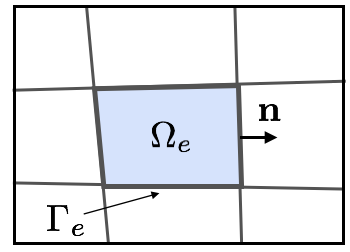
\includegraphics[width=1.5in]{figures/DG_domain.png}
\label{fig:spatial_discretization/dg_domain}}
\subfigure[Element $\Omega_e$]{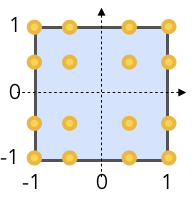
\includegraphics[width=1.5in]{figures/DG_element.png}
\label{fig:spatial_discretization/dg_element}}
\end{center}
\caption{The (a) global domain and (b) element ($N=3$) for the DG method.}
\label{fig:spatial_discretization/dg_method}
\end{figure}

To construct discrete approximations of continuous differential operators (e.g., gradient, divergence, or curl) with the DG method, we first must represent the state vector $\vec{Y}$ using a polynomial representation.  That is, we represent the state vector inside of each element $\Omega_e$ as
\be
\vec{Y}^{(e)}_N(\vec{x},t) = \sum_{i=1}^{M_N} \psi_i(\vec{x}) \vec{Y}^{(e)}_i(t),
\label{eq:spatial_discretization/dg_method}
\ee
where $\psi(\vec{x})$ are the known basis functions and $\vec{Y}^{(e)}_i(t)$ is the solution at each degree of freedom, which is time-dependent. The superscript $(e)$ represents the specific element we are working with, and $i=1,\ldots,M_N$ labels degrees of freedom inside each element $\Omega_e$.  Figure \ref{fig:spatial_discretization/dg_domain} shows a sample global domain, with one specific element $\Omega_e$ identified.  We then map the element from its physical space to the reference element presented in Fig.\ \ref{fig:spatial_discretization/dg_element}; in this particular example $M_N=(N+1)^2$ where $N=3$, which means we are using 3rd-degree polynomials in each direction (yielding 4th-order accuracy).  In general, $N$ need not be constant in each direction, and so we can also write $M_N=(N_{\xi}+1)(N_{\eta}+1)$ in two dimensions or $M_N=(N_{\xi}+1)(N_{\eta}+1)(N_{\zeta}+1)$ in three dimensions, where $\xi$ is along the horizontal direction, $\eta$ along the vertical, and $\zeta$ coming out of the page. 

The attraction of using basis functions $\psi$ to represent the solution $\vec{Y}$ is that computing the gradient of $\vec{Y}$ now only requires applying the gradient operator directly to Eq.~\eqref{eq:spatial_discretization/dg_method}, which yields
\be
\nabla \vec{Y}^{(e)}_N(\vec{x},t) = \sum_{i=1}^{M_N} \nabla \psi_i(\vec{x}) \vec{Y}^{(e)}_i(t),
\label{eq:spatial_discretization/dg_method/gradient}
\ee
where we are able to construct $\grad \psi$ \emph{a priori} since we have chosen the basis functions $\psi$ not to depend on time.

\subsubsection{DG Representation of Conservation Laws}
To describe the DG method, let us describe how one would represent the divergence operator for the conservation law
\be
\diff{\vec{Y}}{t} + \nabla \cdot \Fvector = 0,
\label{eq:spatial_discretization/DG_divergence/conservation_law}
\ee
where, in two dimensions, the flux has components $\Fvector=F_x \wh{\vec{i}} + F_y \wh{\vec{j}}$.
To construct a discrete approximation to Eq.~\eqref{eq:spatial_discretization/DG_divergence/conservation_law}, we first multiply by a test function $\psi_i$ and integrate within each element $\Omega_e$ to arrive at the Galerkin problem statement: find $\vec{Y}^{(e)}_N \in L^2$ such that
\be
\inte \psi_i \diff{\vec{Y}^{(e)}_N}{t} d\Omega_e + \inte \psi_i \nabla \cdot \vecFe_N d\Omega_e= 0 \; \; \forall \; \; \psi \in L^2.
\label{eq:spatial_discretization/DG_divergence/conservation_law/discrete}
\ee
Using the product rule, the second term can be written as 
\be
\inte \psi_i \diff{\vec{Y}^{(e)}_N}{t} d\Omega_e + \inte \nabla \cdot \left( \psi_i \vecFe_N \right) d\Omega_e - \inte \nabla \psi_i \cdot \vecFe_N d\Omega_e= 0.
\label{eq:spatial_discretization/DG_divergence/conservation_law/discrete2}
\ee
Invoking the divergence theorem for the second term yields
\be
\inte \psi_i \diff{\vec{Y}^{(e)}}{t} d\Omega_e + \intb \psi_i \nvector \cdot \vecFe_N d\Gamma_e - \inte \nabla \psi_i \cdot \vecFe_N d\Omega_e= 0,
\label{eq:spatial_discretization/DG_divergence/conservation_law/discrete3}
\ee
where $\Gamma_e$ is the boundary of the element $\Omega_e$ and $\nvector$ is its outward pointing normal vector. We now need to fix the inconsistency of the second term above because it says that the solution along each element boundary $\Gamma_e$ is different from its neighbor since $\vecFe_N$ is allowed to be discontinuous across element boundaries (i.e., if $\vecFe_N \in C^1$ then no such inconsistency would exist).  To fix this, we introduce a numerical flux such that what flows from element $\Omega_e$ to its neighbor $\Omega_k$ is the negative of what flows from $\Omega_k$ into $\Omega_e$.  We represent this fix as follows
\be
\inte \psi_i \diff{\vec{Y}^{(e)}_N}{t} d\Omega_e + \intb \psi_i \nvector \cdot \Fvector^{(*,e)}_N d\Gamma_e - \inte \nabla \psi_i \cdot \vecFe_N d\Omega_e= 0,
\label{eq:spatial_discretization/DG_divergence/conservation_law/discrete4}
\ee
where $\Fvector^{(*,e)}_N$ is the numerical flux that takes into account the solution at $\Omega_e$ and all its neighbors $\Omega_k$ represented by $\Gamma_e$.  In two dimensions, we will have 4 face neighbors and in three dimensions we will have 6 face neighbors.  At this point, one is free to choose their favorite numerical flux just as one would do in the finite-volume method (e.g., Rusanov, Roe, HLL, HLLC, etc.).  Note that it is the numerical flux term that couples all of the equations together; the rest of the terms are completely local within the element.

\subsubsection{Tensor Product Basis Functions}
In Eq.\ \eqref{eq:spatial_discretization/dg_method}, we have said very little about the basis functions $\psi$ and have written the approximation in so-called monolithic form whereby all the degrees of freedom within an element are written as one long vector of length $M_N$.  This way of representing Eq.\ \eqref{eq:spatial_discretization/dg_method} allows for a quick explanation of the DG method but does not illustrate how the method is constructed when tensor product basis functions are used.  In the case of tensor product basis functions, we rewrite $\psi$ (in 2D) as 
\[
\psi_i(\xi,\eta) = h_j(\xi) \otimes h_k(\eta),
\]
where $h$ are one-dimensional basis functions, $\otimes$ denotes the tensor (or Kronecker) product, and $j=1,\ldots N_{\xi}+1$, $k=1,\ldots,N_{\eta}+1$, and $i=j + (k-1) \left( N_{\xi}+1 \right)$. Using this strategy, we can now rewrite Eq.\ \eqref{eq:spatial_discretization/dg_method} as 
\be
\vec{Y}^{(e)}_N(\xi,\eta,t) = \sum_{i=1}^{N_{\xi}+1} \sum_{j=1}^{N_{\eta}+1} h_i(\xi) h_j(\eta) \vec{Y}^{(e)}_{ij}(t),
\label{eq:spatial_discretization/dg_method/tensor-product}
\ee
where we have written the approximation in terms of the reference element coordinates $(\xi,\eta)$ instead of the physical coordinates $(x,y)$.  The advantage of doing this is that the reference element and its coordinates never change, which means that we can use one set of basis functions for all of the elements in the mesh.  

Taking the gradient of Eq.\ \eqref{eq:spatial_discretization/dg_method/tensor-product} yields
\be
\diff{}{\vec{x}} \vec{Y}^{(e)}_N(\xi,\eta,t) = \diff{}{\vec{x}} \sum_{i=1}^{N_{\xi}+1} \sum_{j=1}^{N_{\eta}+1} h_i(\xi) h_j(\eta) \vec{Y}^{(e)}_{ij}(t)
\label{eq:spatial_discretization/dg_method/tensor-product/gradient}
\ee
where $\vec{x}$ can represent either $x$ or $y$.  Let us look at each component separately. Invoking the chain rule yields
\[
\diff{}{x}=\diff{}{\xi} \diff{\xi}{x} + \diff{}{\eta} \diff{\eta}{x}
\]
and
\[
\diff{}{y}=\diff{}{\xi} \diff{\xi}{y} + \diff{}{\eta} \diff{\eta}{y}
\]
where the metric terms $\partial\vec{\xi}/\partial\vec{x}$ need to be computed for each element in the mesh.
Using these we can now rewrite Eq.\ \eqref{eq:spatial_discretization/dg_method/tensor-product/gradient} for the $x$-derivative as 
\be
\diff{}{x} \vec{Y}^{(e)}_N(\xi,\eta,t) = \sum_{i=1}^{N_{\xi}+1} \sum_{j=1}^{N_{\eta}+1} \left( \diff{h_i(\xi)}{\xi}\diff{\xi}{x} h_j(\eta) + h_i(\xi) \diff{h_j(\eta)}{\eta}\diff{\eta}{x} \right) \vec{Y}^{(e)}_{ij}(t).
\label{eq:spatial_discretization/dg_method/tensor-product/x-deriv}
\ee
If we use the same polynomial order along $\xi$ and $\eta$ (call it $N$) then we can simplify Eq.\ \eqref{eq:spatial_discretization/dg_method/tensor-product/x-deriv} to
\be
\diff{}{x} \vec{Y}^{(e)}_N(\xi,\eta,t) = \sum_{i=1}^{N+1} \sum_{j=1}^{N+1} \left( dh_i \xi_x h_j + h_i dh_j \eta_x \right) \vec{Y}^{(e)}_{ij}(t).
\label{eq:spatial_discretization/dg_method/tensor-product/x-deriv2}
\ee
where $h$ is the basis function and $dh$ is its derivative, which are the same functions used along both directions $\xi$ and $\eta$; the index $(i,j)$ will account for which direction we are referring to.

This strategy readily extends to three-dimensions where we write the basis functions as 
\[
\psi_i(\xi,\eta,\zeta) = h_j(\xi) \otimes h_k(\eta) \otimes h_l(\zeta)
\]
with $j=1,\ldots N_{\xi}+1$, $k=1,\ldots,N_{\eta}+1$, $l=1,\ldots,N_{\zeta}+1$, and $i=j + (k-1) \left( N_{\xi}+1 \right) + (j-1)(k-1) \left( N_{\xi}+1 \right)\left( N_{\eta}+1 \right)$. Using this strategy we can rewrite Eq.\ \eqref{eq:spatial_discretization/dg_method} as 
\be
\vec{Y}^{(e)}_N(\xi,\eta, \zeta, t) = \sum_{i=1}^{N_{\xi}+1} \sum_{j=1}^{N_{\eta}+1} \sum_{k=1}^{N_{\zeta}+1} h_i(\xi) h_j(\eta) h_k(\zeta) \vec{Y}^{(e)}_{ijk}(t),
\label{eq:spatial_discretization/dg_method/tensor-product-3d}
\ee
where we have written the approximation in terms of the reference element coordinates $(\xi,\eta, \zeta)$ instead of the physical coordinates $(x,y,z)$. 

Taking the gradient of Eq.\ \eqref{eq:spatial_discretization/dg_method/tensor-product-3d} yields
\be
\diff{}{\vec{x}} \vec{Y}^{(e)}_N(\xi,\eta,\zeta,t) = \diff{}{\vec{x}} \sum_{i=1}^{N_{\xi}+1} \sum_{j=1}^{N_{\eta}+1} \sum_{k=1}^{N_{\zeta}+1} h_i(\xi) h_j(\eta) h_k(\zeta) \vec{Y}^{(e)}_{ijk}(t).
\label{eq:spatial_discretization/dg_method/tensor-product-3d/gradient}
\ee
Taking each component separately and invoking the chain rule yields
\[
\diff{}{x}=\diff{}{\xi} \diff{\xi}{x} + \diff{}{\eta} \diff{\eta}{x} + \diff{}{\zeta} \diff{\zeta}{x},
\]
\[
\diff{}{y}=\diff{}{\xi} \diff{\xi}{y} + \diff{}{\eta} \diff{\eta}{y} + \diff{}{\zeta} \diff{\zeta}{y},
\]
and
\[
\diff{}{z}=\diff{}{\xi} \diff{\xi}{z} + \diff{}{\eta} \diff{\eta}{z} + \diff{}{\zeta} \diff{\zeta}{z},
\]
where the metric terms $\diff{\vec{\xi}}{\vec{x}}$ need to be computed for each element in the mesh.
Using these we can now rewrite Eq.\ \eqref{eq:spatial_discretization/dg_method/tensor-product-3d/gradient} for the $x$-derivative as follows
\begin{multline}
 \diff{}{x} \vec{Y}^{(e)}_N(\xi,\eta,t) =  \sum_{i=1}^{N_{\xi}+1} \sum_{j=1}^{N_{\eta}+1} \sum_{k=1}^{N_{\zeta}+1} \\ 
 \left( \diff{h_i(\xi)}{\xi}\diff{\xi}{x} h_j(\eta) h_k(\zeta) + h_i(\xi) \diff{h_j(\eta)}{\eta}\diff{\eta}{x} h_k(\zeta) 
 + h_i(\xi) h_j(\eta) \diff{h_k(\zeta)}{\zeta}\diff{\zeta}{x} \right) \vec{Y}^{(e)}_{ijk}(t) .
\label{eq:spatial_discretization/dg_method/tensor-product-3d/x-deriv}
\end{multline}
If we use the same polynomial order along $\xi$, $\eta$, and $\zeta$ then we can simplify Eq.\ \eqref{eq:spatial_discretization/dg_method/tensor-product-3d/x-deriv} as follows
\be
\diff{}{x} \vec{Y}^{(e)}_N(\xi, \eta, \zeta, t) = \sum_{i=1}^{N+1} \sum_{j=1}^{N+1} \sum_{k=1}^{N+1} \left( dh_i \xi_x h_j h_k + h_i dh_j h_k \eta_x + h_i h_j dh_k \zeta_x\right) \vec{Y}^{(e)}_{ijk}(t).
\label{eq:spatial_discretization/dg_method/tensor-product-3d/x-deriv2}
\ee
where the index $(i,j,k)$ will account for which direction we are referring to.

\subsubsection{Implementation}

\hl{[Frank/Lucas/Jeremy: Can we write a little here about the implementation, to make it easier for people to connect the code with what is written above? For example, how are boundary conditions implemented?]} 
[\fxg{Tapio, perhaps we can discuss this on Friday to understand what you are looking for exactly here.}]

\subsection{Time-Discretization Methods}\label{s:timestepping}

\subsubsection{Additive Runge-Kutta IMEX Methods}

To circumvent the time-step restriction due to the fast acoustic waves, we rely on implicit-explicit (IMEX) methods. For the LES model, if the aspect ratio of the horizontal to vertical grid spacing is near unity, it is beneficial to use fully 3D-IMEX methods.  For the global atmospheric model with large aspect ratios of grid elements, we use 1D-IMEX methods in which the time-integrator is fully explicit in the horizontal direction (HE) and implicit in the vertical direction (so-called HEVI schemes).

We use a general family of additive Runge-Kutta methods (ARK) methods for both the 1D and 3D IMEX approaches (see, e.g., \citet{giraldo:2013}). Note that adding fully-implicit Runge-Kutta (IRK) methods to the 3D-IMEX approach is quite trivial, so this can be included as an option. Fully-implicit methods have no time-step restriction with respect to stability.

To get a sense of how the ARK approach works, let us describe a general abstract model here that will be used in later sections to describe specific formulations. To describe the abstract IMEX formulation, let us partition the total tendency $\vec{\mathcal{T}}$ on the right-hand side of Eq.~\eqref{e:eom_compact} into four process speeds,
\[
\frac{\partial \vec{Y}}{\partial t} = \Tvector = - \nabla \cdot \Fvector + \vec{\mathcal{S}} = \Tvector_{\mathrm{fastest}} + \Tvector_{\mathrm{fast}} + \Tvector_{\mathrm{dynamical}} + \Tvector_{\mathrm{slow}}.
\]
Let us further partition the tendency $\Tvector_\mathrm{fastest}$ containing the fastest waves in the system into a component linear in state variables and a residual nonlinear component,
\[
\Tvector_\mathrm{fastest} =  \Tvector^L_\mathrm{fastest} \qvector + \Tvector^N_\mathrm{fastest}(\qvector).
\]
This then allows us to write the semi-discrete form (in space) as follows
\begin{equation}\label{eq:IMEX}
\difft{\qvector}{t} =  \Tvector^L_\mathrm{fastest} \qvector + \Tvector_\mathrm{fast} + 
\Tvector_\mathrm{dynamical} + \Tvector^N_\mathrm{fastest}(\qvector) + \Tvector_\mathrm{slow}.
\end{equation}
To discretize the equations in time, we first compute the stage values
\begin{multline}\label{eq:IMEX/stages}
\qstage^{(i)}= \qvector^n + \Delta t \sum_{j=0}^{i} \left( a^{\mathrm{fastest}}_{ij} \Tvector_{\mathrm{fastest}}^L \qstage^{(j)} \right) + \Delta t \sum_{j=0}^{i-1} \left( {a}^{\mathrm{fast}}_{ij} \Tvector_{\mathrm{fast}}(\qstage^{(j)}) \right)  \\
+  \Delta t \sum_{j=0}^{i-1} \left( {a}^{\mathrm{dynamical}}_{ij} \bigl(\Tvector_{\mathrm{dynamical}}(\qstage^{(j)}) + \Tvector^N_\mathrm{fastest}(\qstage^{(j)})\bigr)\right) \\
+ \Delta t \sum_{j=0}^{i-1} \left( {a}^{\mathrm{slow}}_{ij} \Tvector_{\mathrm{slow}}(\qstage^{(j)}) \right)
\end{multline}
with $i=1,\ldots,s$ representing the $s$ stages, $\qstage^{(0)}=\qvector^n$ (where $\qvector^n$ is the solution vector at the current time), and $a$ are the coefficients of the partitioned Butcher tableau (see, e.g., \citet{constantinescu:2007, constantinescu:2007}). Here, the nonlinear component of the fastest term was assumed to evolve with other terms on dynamical timescales. Some rows of the coefficient matrices $a$ for the slower component will be zero. \hl{\textbf{Frank}: We need to write this in a way that facilitates implementation, potentially with more subdivisions of a timestep. It makes sense to me to subcycle the faster components by an integer multiple of the dynamical timestep, and correspondingly to superstep the slow components by another integer multiple. Can we write this out explicitly now, even without having the Butcher tableaus worked out? As I mentioned, we need this immediately once IMEX works and need to work on the implementation aspects now.} 
[\fxg{I have a call scheduled with Mark Taylor next week. We have been discussing what they are doing in E3SM and has sent me new papers on this.  Right now, they are using explicit time-integration only but are moving to semi-Lagrangian with a fixer for the mass.}]
The solution at time $n+1$ is obtained from
\be
\qvector^{n+1}=\qvector^n + \Delta t \sum_{i=0}^{s} \left( b_i \vec{\mathcal{T}}(\qstage^{(i)}) \right).
\label{eq:IMEX/update}
\ee
So far we have defined a diagonally-implicit Runge-Kutta (DIRK) method \citep{alexander:1977,butcher:1981a,ascher:1997,boscarino:2009}.  To make the DIRK more efficient, we impose the restriction that all diagonal values $\wt{a}_{ii}$ are constant. This allows one construction of the matrix problem that does not change across stage values.  This we now refer to as singly-diagonally-implicit Runge-Kutta (SDIRK).

Rearranging Eq.\ \eqref{eq:IMEX/stages} as follows
\begin{multline}\label{eq:IMEX/stages2}
\left( \vec{I} - {a}^{\mathrm{fastest}}_{ii}\Tvector^L_{\mathrm{fastest}} \right)  \qstage^{(i)}  =  \qvector^n + 
\Delta t \sum_{j=0}^{i-1} \left( {a}^{\mathrm{fast}}_{ij} \Tvector_{\mathrm{fast}}(\qstage^{(j)}) \right)   \\
+ \Delta t \sum_{j=0}^{i-1} \left( {a}^{\mathrm{dynamical}}_{ij} \bigl(\Tvector_{\mathrm{dynamical}}(\qstage^{(j)}) + \Tvector^N_\mathrm{fastest}(\qstage^{(j)})\bigr) \right) \\
+ \Delta t \sum_{j=0}^{i-1} \left( {a}^{\mathrm{slow}}_{ij} \Tvector_{\mathrm{slow}}(\qstage^{(j)}) \right) 
\end{multline}
reveals the implicit nature of the problem. Letting $\vec{A}=\vec{I} - {a}^{\mathrm{fastest}}_{ii} \Tvector^L_{\mathrm{fastest}}$, $\vec{X}=\qstage^{(i)}$, and denoting the right-hand side of Eq.~\eqref{eq:IMEX/stages2} by $\mathcal{B}$, we obtain the linear system 
\[
\vec{A} \vec{X} = \mathcal{B}.
\]
We can solve this linear system using, e.g., Krylov subspace methods such as GCR or GMRES (we cannot use conjugate gradient since the system is hyperbolic and therefore is not symmetric positive-definite in the current form). ARK of order $\order(\Delta ^k)$ for $k=2,\ldots,5$ are planned (which are roughly of order $k=s-1$ where $s$ denotes the number of stages.

\subsubsection{Reference State for Linearization}

\hl{TODO in code: Implement the reference state calculation for an arbitrary $T_r(z)$; constant $T_r$ for now is fine.}

Solving for the fastest waves implicitly by a linear solve requires linearization of the fastest tendency terms. We generally use reference states characterized by a temperature $T_r(z)$ that may depend on height $z$ but does not depend on horizontal coordinates. We enforce hydrostatic balance, and assume the reference state is dry, so that the reference pressure is obtained by combining hydrostatic balance ($\partial_z p_r(z) = - \rho_r g$) with the ideal gas law ($p_r=R_d \rho_r T_r$), giving 
\[
p_r(z) = p_{\mathrm{MSLP}} \exp\left(-\int_0^z \frac{dz}{H(z)} \right),
\]
where
\[
H(z)  = \frac{R_d T_r(z)}{g}
\]
is the scale height and we chose for $p_r(0)$ the mean sea level pressure $p_{\mathrm{MSLP}}$. For the simple and commonly used choice of a constant reference temperature $T_r$, this reduces to
\begin{equation}
    p_r = \exp (-z/H),
\end{equation}
where the scale height $H = R_d T_{r}/g$ is constant. The reference density then follows from the ideal gas law as
\begin{equation}
    \rho_r = \frac{p_r}{R_d T_{r}}.
\end{equation}

Because the reference temperature and thus the reference pressure are assumed to be constant in the horizontal, the reference state is assumed at rest, $\vec{u}_r = 0$, consistent with geostrophic balance. Because the reference state is assumed dry, $q_k= 0$ for $k \in \{ t, v, l, i, p\}$ in the reference state.

More sophisticated reference states for linearization are possible, for example, with a latitudinally varying hydrostatically balanced temperature profile, and with a reference state velocity in geostrophic and hydrostatic balance with this temperature field. 
 
 \subsubsection{3D-IMEX Approach}
 \label{sec:3D-IMEX/v1}
If the grid aspect ratio between the horizontal $\Delta_h$ and the vertical $\Delta_v$ is near unity, $\Delta_h/\Delta_v \approx 1$, the stiffness of the equations arises from the acoustic modes (i.e., sound waves), which travel along all three spatial dimensions. In this case, we must extract the acoustic waves in all three spatial dimensions and treat them implicitly.  

To linearize, we introduce the following splitting: $\rho(\vec{x},t)=\rho_r(\vec{x}) + \rho'(\vec{x},t)$,  $p(\vec{x},t)=p_r(\vec{x}) + p'(\vec{x},t)$, and $(\rho \etotal)'=\rho \etotal - \rho_r e_r$, where the terms $\vec{Y}'(\vec{x},t)=\vec{Y}(\vec{x},t)-\vec{Y}_r(\vec{x})$ denote perturbation variables from the reference state  $\vec{Y}_r$, assumed to be at rest with $\vec{u}_r = 0$.
 
Let us assume the fastest tendency terms $\Tvector_{\mathrm{fastest}}$ contain contributions from advection, pressure terms, some source terms, so that sound waves are captured:
 \[
 \Tvector_{\mathrm{fastest}}=-\nabla \cdot \left( \Fadv_{\mathrm{fastest}} + \Pvector_{\mathrm{fastest}}\right) + \Source_{\mathrm{fastest}}.
 \]
The linear components of the relevant flux terms in Eqs.\ \eqref{e:adv_flux}--\eqref{eq:diff_flux} can be written as follows (with $\mathcal{L}(\cdot)$ denoting the linear component): 
 \begin{equation}
 \mathcal{L}\left(\Fadv_{\mathrm{fastest}}\right)=\left( \begin{array}{c}
 \left(\rho \vec{u}\right) \\
 \vec{0} \\
 e_r \left(\rho \vec{u}\right)\\
\vec{0}\\
\vec{0} \\
\vec{0}
\end{array}
\right), 
\qquad
\mathcal{L}\left(\Pvector_{\mathrm{fastest}}\right)= \left( \begin{array}{c}
\vec{0} \\
p' \vec{I}_3 \\
\frac{p_r}{\rho_r} \left( \rho \vec{u}\right)\\
\vec{0} \\
\vec{0} \\
\vec{0} 
\end{array}
\right)
\label{eq:fluxes_linear}
\end{equation}
And the linear component of the source term \hl{[So you are including external gravity waves  in the implicit part, too, in contrast to what is stated at the beginning of the section? Do we really want to do that? It seems unusual for LES.]}
[\fxg{The way this section was initially written represented what we COULD do.  I am now modifying this section to reflect what is actually done in the code.}] \hl{[Well, we need to know what we actually should implement.]}
is 
\begin{equation}
\mathcal{L}\left( \Source_{\mathrm{fastest}}\right) = \left( \begin{array}{c}
 0 \\
 - \rho' \nabla\Phi  \\
0 \\
0 \\
0 \\
0
\end{array}
\right)
\end{equation}
which is linear with respect to $\rho'$. To obtain a system that is linear in state variables, we also need to express the perturbation  pressure $p'= p - p_r$ as a linear function of state variables. We can do so by first computing the linearized internal energy perturbation per unit volume,
\begin{equation}
(\rho I)' \approx (\rho \etotal)'  -  \rho' \Phi,
\end{equation}
assuming a reference state at rest, and computing from that the perturbation product of density and temperature
using a version of the temperature equation~\eqref{eq:temperature} that is linear in the state variables:
\begin{equation}\label{eq:temperature_perturb}
(\rho T)' =  \frac{(\rho I)'  - (\rho q_t - \rho q_l)I_{v,0} + (\rho q_i) (I_{i,0} + I_{v,0})}{c_{vd}}.
\end{equation}
The ideal gas law (neglecting moisture perturbations affecting the gas constant) then gives the perturbation pressure
\begin{equation}\label{eq:pressure_perturb}
\begin{split}
p' & \approx R_d (\rho T)' \\
   & \approx \frac{R_d}{c_{vd}} \bigl[ (\rho I)'  - (\rho q_t - \rho q_l)I_{v,0} + (\rho q_i) (I_{i,0} + I_{v,0}) \bigr].
\end{split}
\end{equation}
This gives the perturbation pressure as a linear function of state variables. 

Defining 
\[
\Tvector^L_{\mathrm{fastest}}  = - \nabla \cdot \left( \mathcal{L} \bigl(\Fadv_{\mathrm{fastest}}\bigr) + \mathcal{L}\left(\Pvector_{\mathrm{fastest}}\right) \right) + \mathcal{L}\left( \Source_{\mathrm{fastest}}\right),
\]
we obtain the nonlinear component of the fastest tendency as the residual 
\[
\Tvector^N_{\mathrm{fastest}} = \Tvector_{\mathrm{fastest}} - \Tvector^L_{\mathrm{fastest}}.
\] 
This allows us to use the IMEX time stepping strategy \eqref{eq:IMEX/stages2}. It yields the maximum eigenvalue of the Jacobian operators  $\lambda_{\mathrm{fastest}}=\widehat{\vec{n}} \cdot \vec{u} + c_{s}$ (corresponding to $\Tvector_{\mathrm{fastest}}$) and  $\lambda^L_{\mathrm{fastest}} = c^L_s$ (corresponding to $\Tvector^L_{\mathrm{fastest}}$), where $c^L_s$ is the speed of sound \eqref{e:soundspeed} \hl{the speed of sound isn't exactly that given by (21) but includes a modification from the stratification of the background state. Not sure it matters, but what is stated here is not exact, even with an isothermal, dry reference state. See discussion of sound waves and gravity waves, e.g., in Durran's book on numerical methods.} in the reference state and $c_s$ is the speed of sound with respect to the total variables. 
 
 \comment{
\subsubsection{3D-IMEX Approach: Version 2}
\label{sec:3D-IMEX/v2}
The advantage of using version 1 presented in Sec.\ \ref{sec:3D-IMEX/v1} is that we can construct the explicit solution of the governing equations and then view the implicit portion of the IMEX method as a correction to the explicit solution.  However, following this approach may cause the discrete form of the equations to lose hyperbolicity (see \cite{bispen:2017}).

To avoid this situation, we split the $\vec{\mathcal{T}}$ operator directly into a linear and nonlinear part:
\begin{equation}
 \vec{\mathcal{T}}(\qvector)=- \left( \begin{array}{c}
 0 \\
 \nabla \cdot (\rho \vec{u} \otimes \vec{u}) \\
 \nabla \cdot ( (E' + p') \vec{u} )
\end{array}
\right) 
+
\left( \begin{array}{c}
 \nabla \cdot (\rho \vec{u} ) \\
 \nabla p'  + \rho' \nabla \Phi \\
 \nabla \cdot ( (E_r + p_r) \vec{u} )
\end{array}
\right).
\label{eq:3d-IMEX/S_operator/split}
\end{equation}
 Here, we have eliminated the reference pressure gradient and reference buoyancy due to, e.g., hydrostatic balance. With this approach, the maximum eigenvalue for the Jacobian operators are $\lambda^{(N)}_{\max}=2 \widehat{\vec{n}} \cdot \vec{u}$ and 
 $\lambda^{(L)}_{\max}= c_s$, where the superscripts (N) and (L) denote the operator that the eigenvalue is associated with.
}

\subsubsection{1D-IMEX Approach}
\label{sec:1D-IMEX}

\hl{[NEED TO FIX THIS SECTION WHEN 3D IS DONE.]}

For grid aspect ratios $\Delta_h/\Delta_v \gg 1$, the stiffness of the equations will arise from the vertically propagating acoustic modes if the explicit CFL number will not be violated in the horizontal. For this situation, we only need to extract acoustic waves along the vertical direction and treat them implicitly.  Following a similar approach for the 3D-IMEX method given in Sec.\ \ref{sec:3D-IMEX/v1}, we write
 \[
\Tvector= \Tvector_{\mathrm{fastest}} + \Tvector_{\mathrm{fast}} + \Tvector_{\mathrm{dynamical}} + \Tvector_{\mathrm{slow}}
\]
%where $\Tvector_{\mathrm{fastest}}=-\nabla \cdot \left( \Fvector_{\mathrm{fastest}} + \Pvector_{\mathrm{fastest}}\right)+ \Source_{\mathrm{fastest}}$
 which must be linear with respect to $\qvector'$. 
 As a first approach, let us define this operator as follows:
 
 \comment{
 \[
 \Tvector_{\mathrm{fastest}}=- \diff{}{z} \left( \Fadv_{\mathrm{fastest}} + \Pvector_{\mathrm{fastest}} + \Fdiff_{\mathrm{fastest}} \right) + \Source_{\mathrm{fastest}}
 \]
 where $z$ here denotes the direction in which gravity acts (in the LES simulations, this is indeed the z-coordinate but on the sphere this is the radial direction which is just the vector along $\vec{x}=x \hat{i} + y \hat{j} + z \hat{k}$).  Let us start with the fluxes given by Eqs.\ \eqref{e:adv_flux}--\eqref{eq:diff_flux} and write their linear representations as follows
 \begin{equation}
 \Fadv_{\mathrm{fastest}}=\left( \begin{array}{c}
 \rho w \\
 0 \\
 0 \\
 0 \\
 \rho_r e_r w\\
0 \\
0 \\
0
\end{array}
\right), 
\Pvector_{\mathrm{fastest}}= \left( \begin{array}{c}
0 \\
0 \\
0 \\
p' \\
p_r w \\
0 \\
0 \\
0 
\end{array}
\right),
\Fdiff_{\mathrm{fastest}}=\left( \begin{array}{c}
 \rho_r \vec{d}_{q_t} \cdot \vec{k} \\
 \rho_r \vec{\tau} \cdot \vec{k} \\
 \rho_r \vec{J} + \rho_r \vec{D} \cdot \vec{k}\\
\rho_r \vec{d}_{q_k} \cdot \vec{k} \\
\rho_r \vec{d}_{q_{p, i}} \cdot \vec{k}\\
\rho_r \vec{d}_{\chi_j} \cdot \vec{k}
\end{array}
\right)
\label{eq:fluxes_linear_1d}
\end{equation}
}

\[
 \Tvector_{\mathrm{fastest}}=- \diff{}{z} \left( \Fadv_{\mathrm{fastest}} + \Pvector_{\mathrm{fastest}} \right) + \Source_{\mathrm{fastest}}
 \]
 where $z$ here denotes the direction in which gravity acts (in the LES simulations, this is indeed the z-coordinate but on the sphere this is the radial direction which is just the vector along $\vec{x}=x \hat{i} + y \hat{j} + z \hat{k}$).  Let us start with the fluxes given by Eqs.\ \eqref{e:adv_flux}--\eqref{eq:diff_flux} and write their linear representations as follows
 \begin{equation}
 \mathcal{L} \left( \Fadv_{\mathrm{fastest}} \right)=\left( \begin{array}{c}
 \left( \rho w \right) \\
 0 \\
 0 \\
 0 \\
 e_r \left( \rho w \right) \\
0 \\
0 \\
0
\end{array}
\right), 
\mathcal{L} \left( \Pvector_{\mathrm{fastest}} \right) = \left( \begin{array}{c}
0 \\
0 \\
0 \\
p' \\
\frac{p_r}{\rho_r} \left( \rho w \right) \\
0 \\
0 \\
0 
\end{array}
\right),
\mathcal{L} \left( \Source_{\mathrm{fastest}} \right) = \left( \begin{array}{c}
0 \\
0 \\
0 \\
\rho' \diff{\phi}{z} \\
0 \\
0 \\
0 \\
0 
\end{array}
\right),
\label{eq:fluxes_linear_1d}
\end{equation}
which are linear with respect to $\rho'$, $\rho w$, and 
$p'=(\gamma-1)\left((\rho \etotal)' - \rho' \phi\right)$ where
$(\rho \etotal)'=(\rho \etotal - \rho_r e_r)$.  The term $\rho w$ represents the momentum along the z-direction (for LES it is indeed the Cartesian component in the vertical but on the sphere it represents the radial momentum component $\frac{\vec{x}}{||\vec{x}||} \cdot \left(\rho \vec{u}\right)$).

\comment{
\begin{equation}
 \Tvector_{\mathrm{fastest}} =- \left( \begin{array}{c}
 \diff{}{z} (\rho w) \\
 \vec{0} \\
 \vec{0} \\
 \diff{p'}{z}  + \rho' \diff{\Phi}{z} \\
 \diff{}{z}\left(  (\rho_r e_r + p_r) w \right) \\
 \vec{0}
\end{array}
\right)
\label{eq:1d-IMEX/L_operator}
\end{equation}
}
With the linear operator
\[
\Tvector^L_{\mathrm{fastest}} = - \diff{}{z} \left( \mathcal{L}\left(\Fadv_{\mathrm{fastest}}\right) + \mathcal{L}\left(\Pvector_{\mathrm{fastest}}\right) \right) + \mathcal{L}\left( \Source_{\mathrm{fastest}}\right)
\]
defined, we can then define the remaining nonlinear operator as 
\[
\Tvector^N_{\mathrm{fastest}} =\Tvector_{\mathrm{fastest}} - \Tvector^L_{\mathrm{fastest}}
\]
and follow the procedure outlined in Sec.\ \ref{sec:3D-IMEX/v1}. 

\section{Topography}
Topography can be either built analytical or by reading an external topography file. The topography data are taken from the NOAA ETOPO-1 database \cite{etopo1}. As of now, only {\bf XYZ files are being read}. If necessary, a NetCFD topograpjhy reader can be easily added.
An example of high order grid built on the topography of the Monterey bay in California is shown in Figure \ref{fig:montereySurfaceGrid}. The high order grid is built so that the elements follow the geometric curvature. A detailed view of the curved high order elements is shown in Figure \ref{fig:gridDetailView}

\begin{figure}[htbp]
\centering
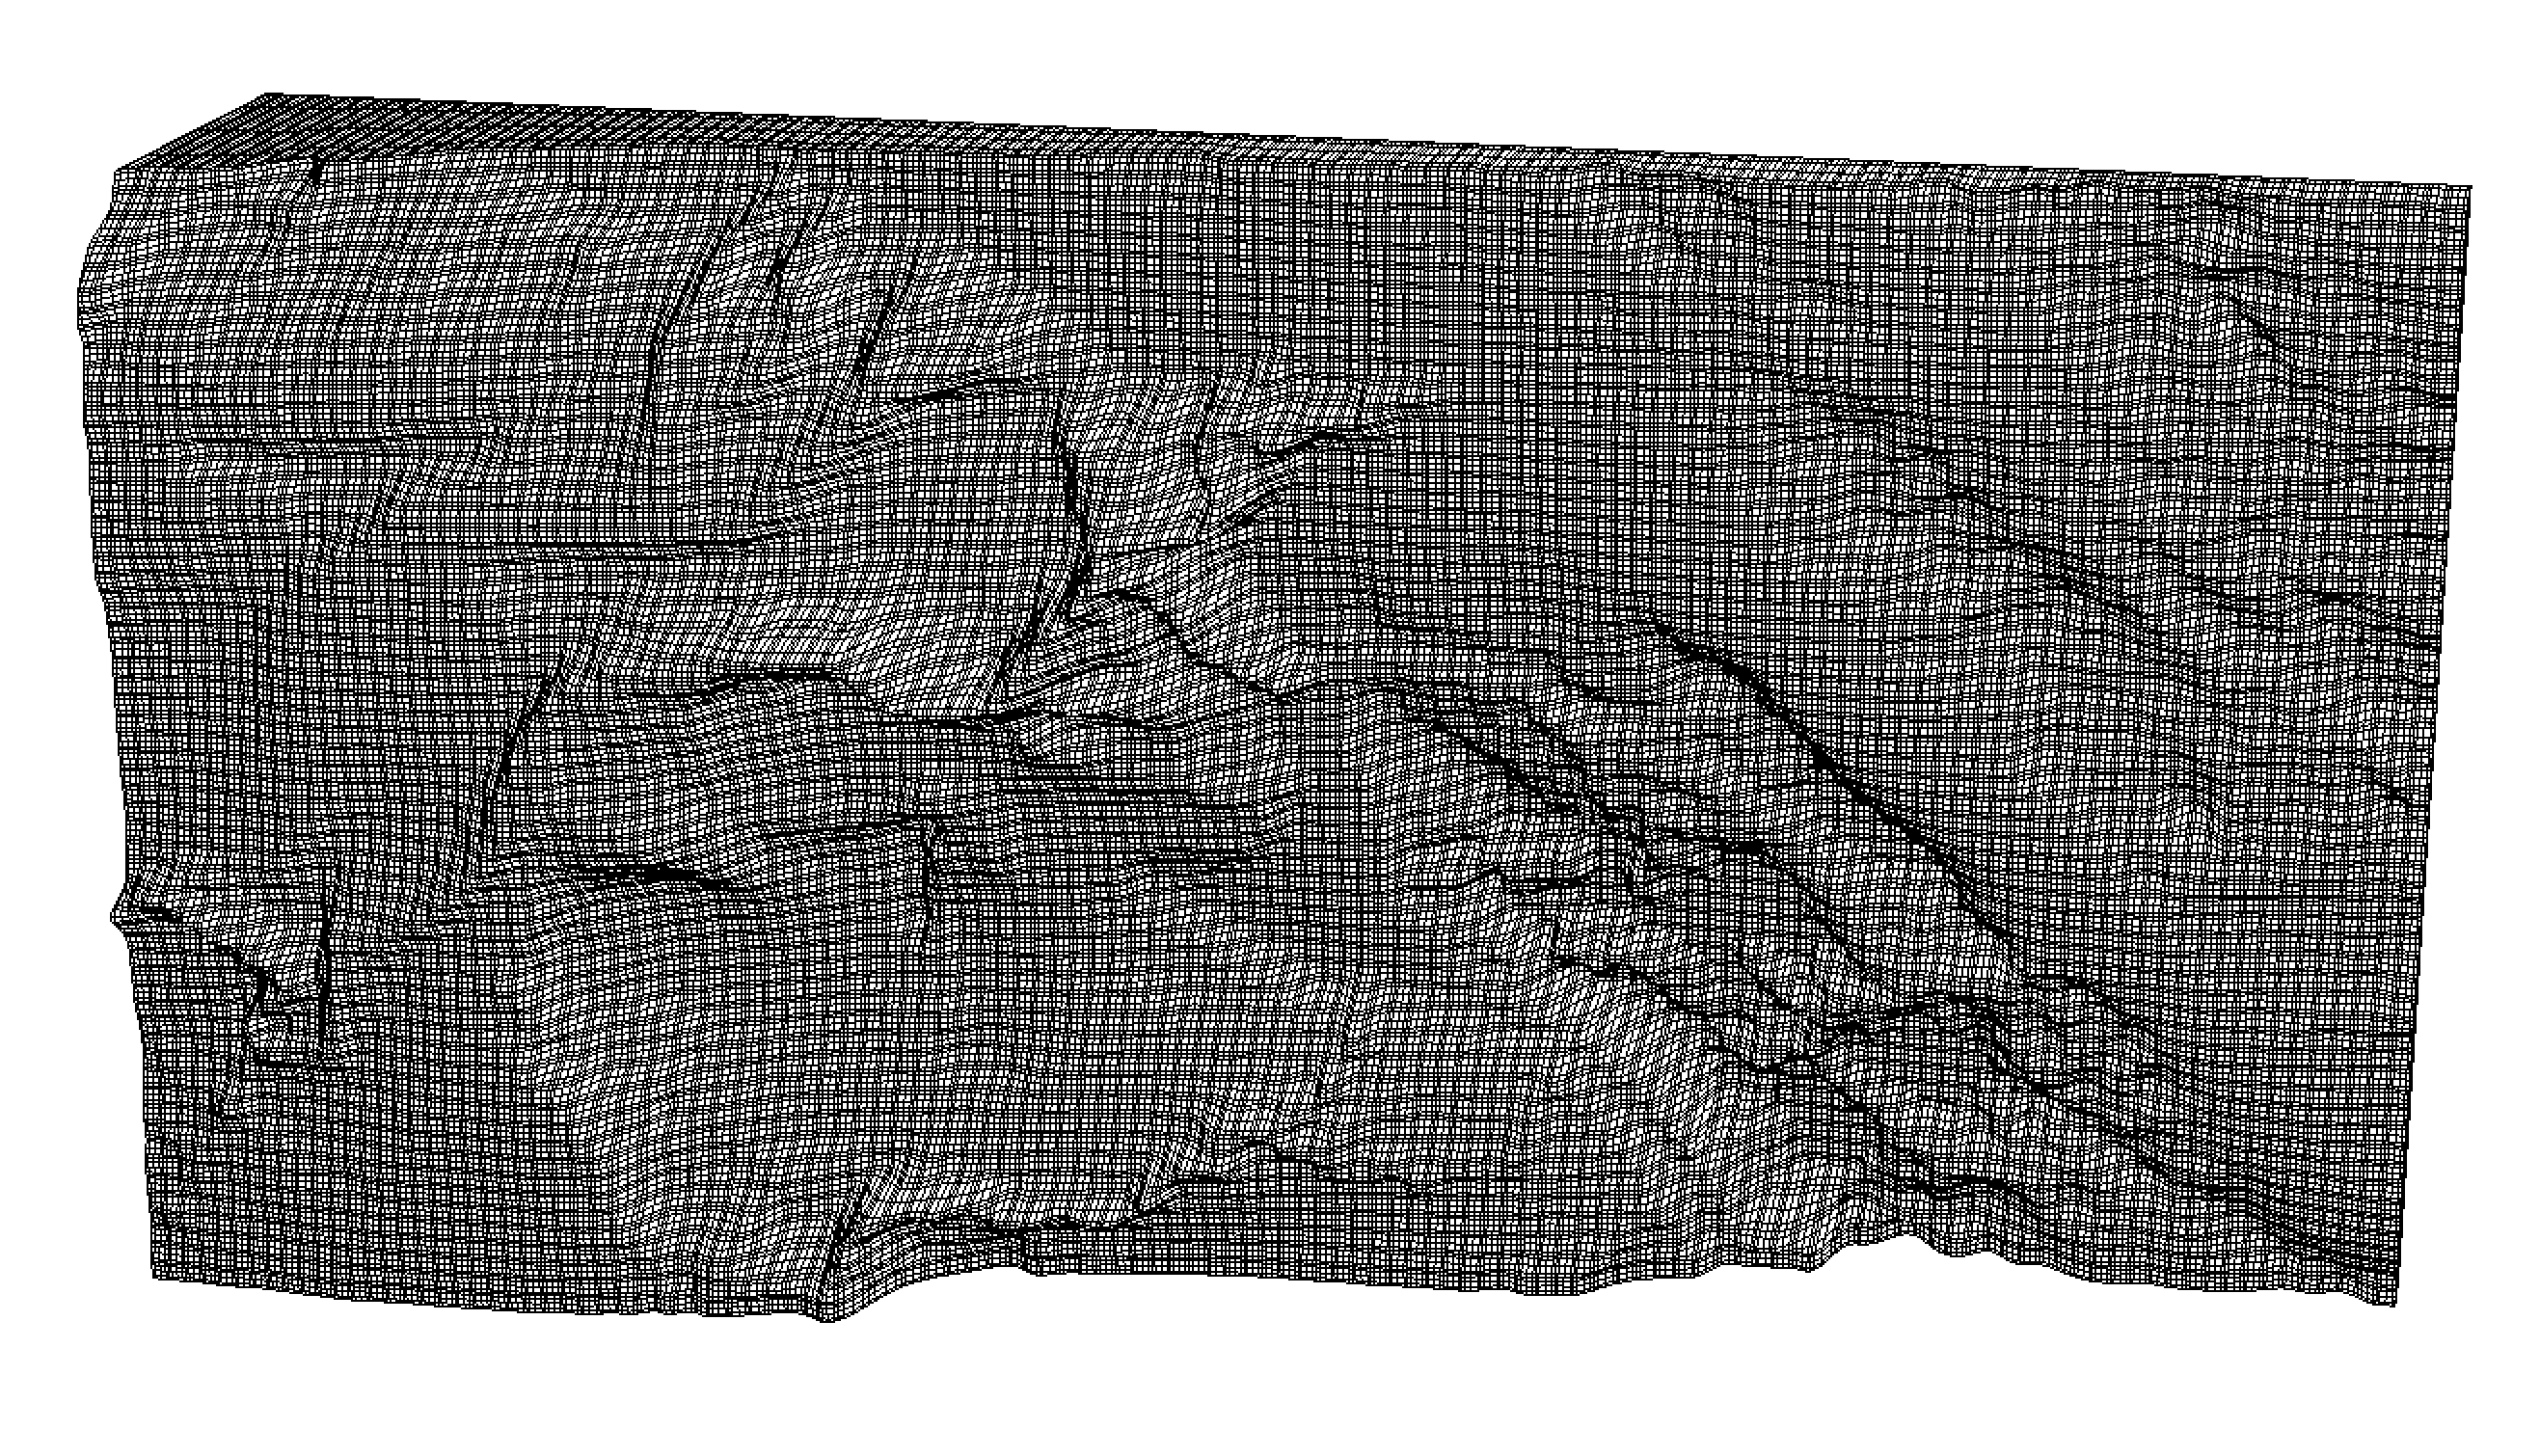
\includegraphics[width=\textwidth]{figures/monterey_with_grid.png}
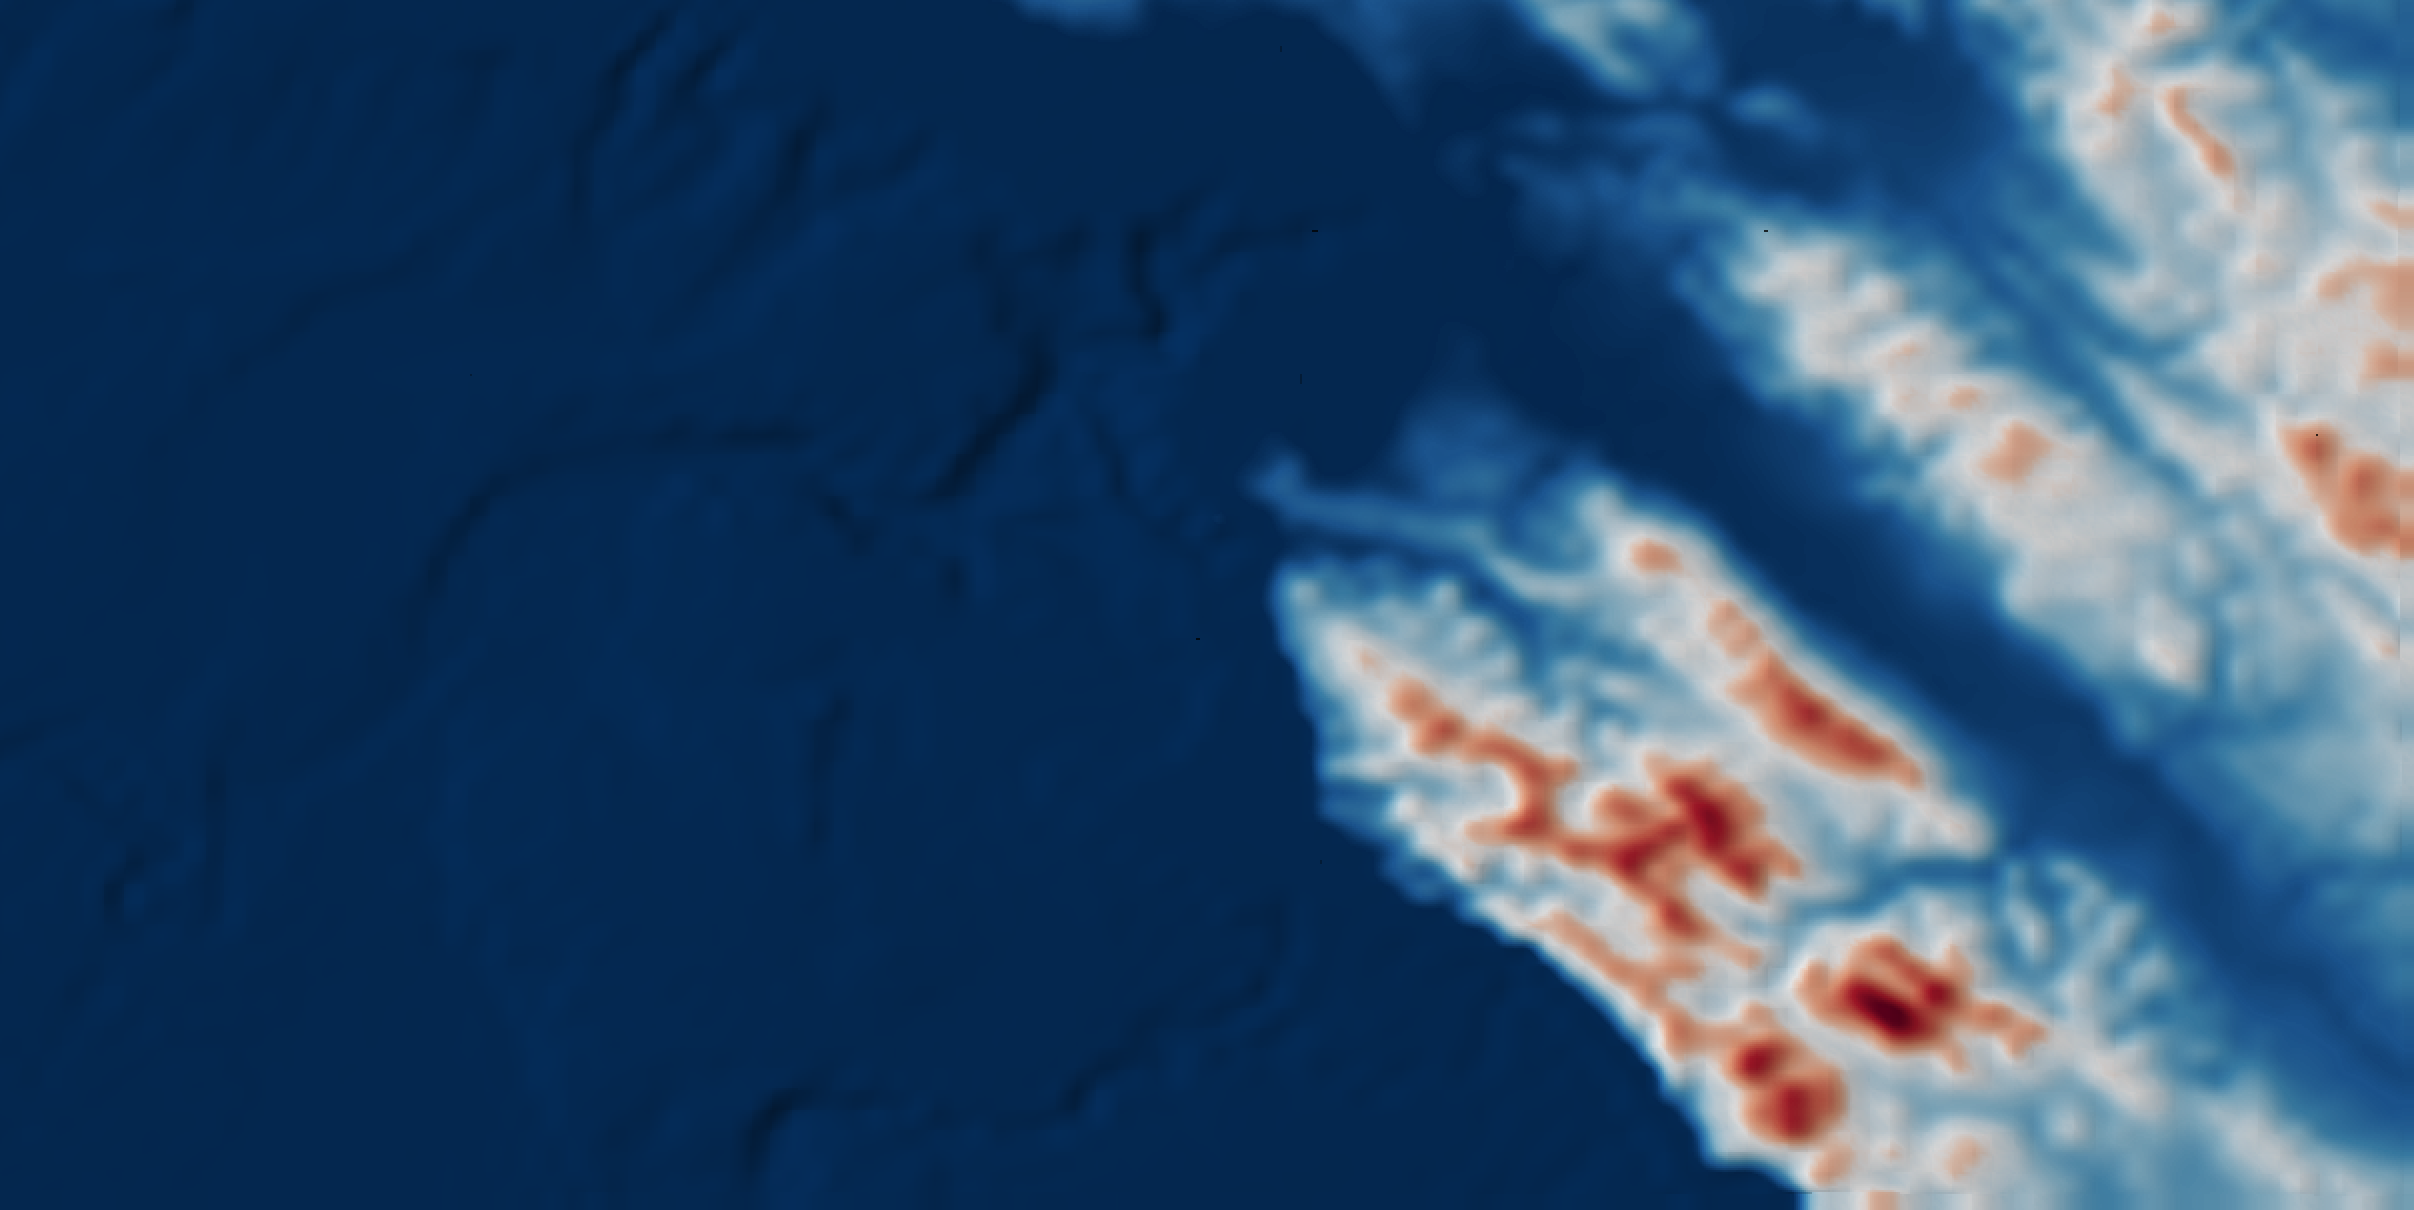
\includegraphics[width=\textwidth]{figures/monterey_colorscale.png}
\caption{Bottom view of the meshed Monterey Bay, California. The high order elements are visible in the top image whereas the topography is colored by its elevation in the bottom.}
\label{fig:montereySurfaceGrid}
\end{figure}

\begin{figure}[htbp]
\centering
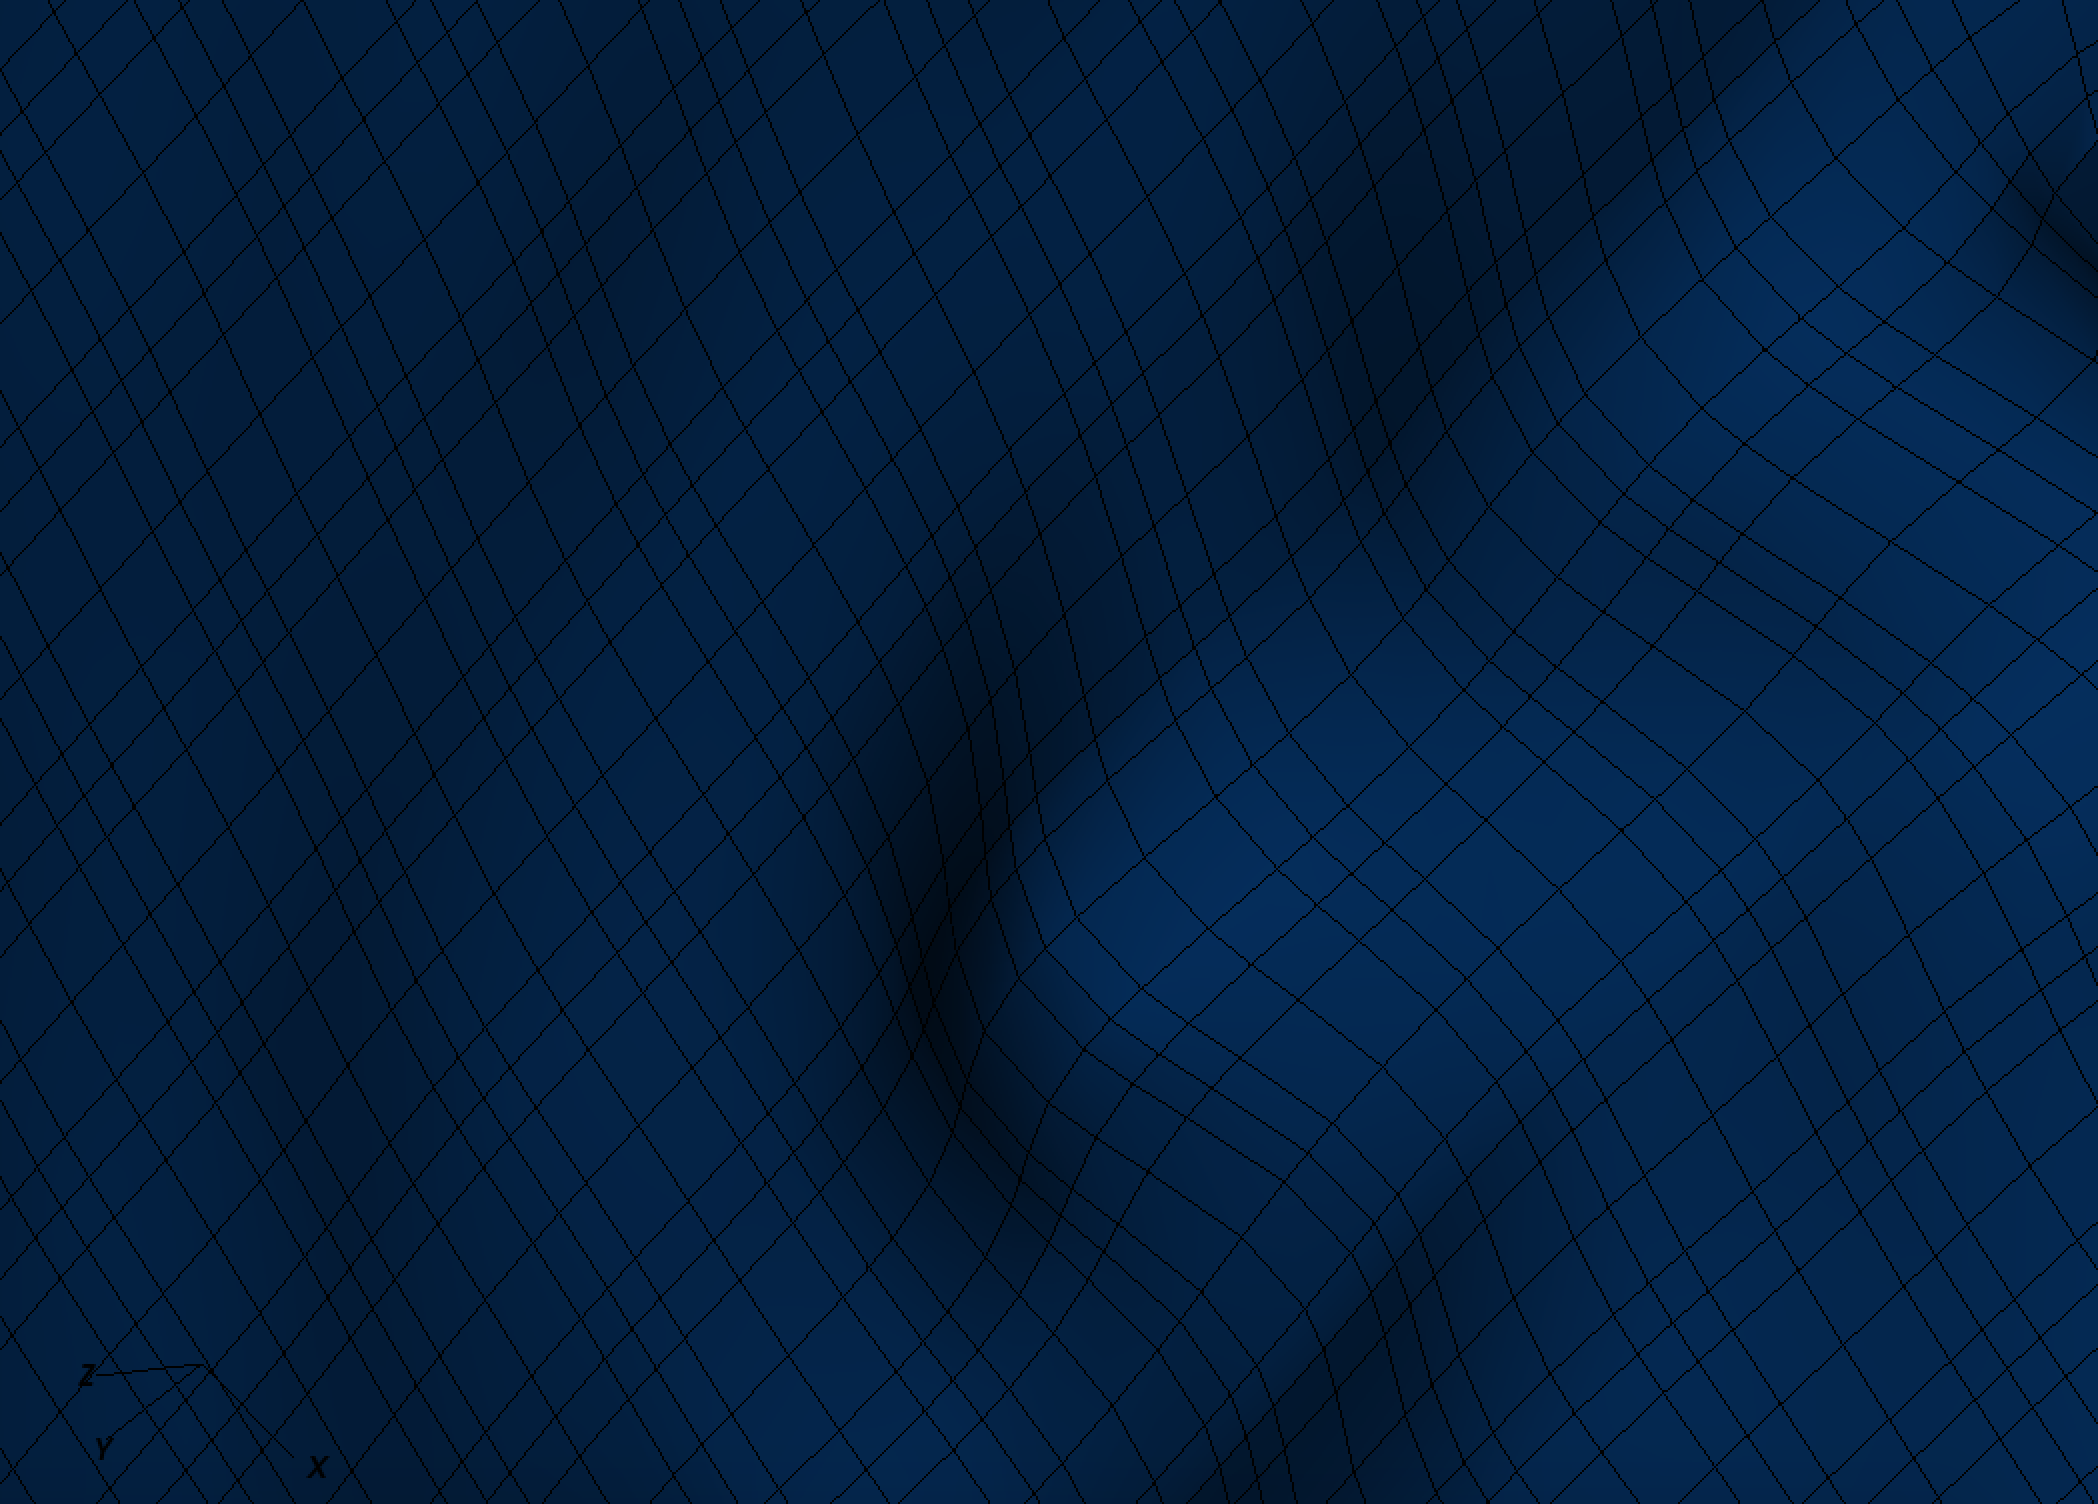
\includegraphics[width=\textwidth]{figures/GRID-detail.png}
\caption{A close view of the curved high order elements on the topography.}
\label{fig:gridDetailView}
\end{figure}

\subsection{Topography files and database}
The external topographic files are not incorporated into the CLIMA repository. 
They are automatically downloaded via a call to {\tt wget} from the {\tt Julia} driver into the user's working directory {\tt \$CLIMA\_HOME/USERS/TEST/DIRECTORY}. As of now, the available topography files are hosted here \url{https://web.njit.edu/~smarras/TopographyFiles} (notice: this directory is not directly accessible from the browser).

\hl{The grid reader should be enhanced to map the grid onto the sphere. As of now, the grid is read and mapped into a closed box only.}

\section{Benchmarking the dynamical core (Dycore)}

\hl{STILL INCOMPLETE}
Here we describe a set of benchmarks for dry and moist atmospheres. The results presented in this document have been assessed against those presented in the literature. 

\subsection{2D rising thermal bubble by Robert 1993}
\label{2dRTBtest}
This test is described \cite{robert1993}. It consists of a flow that is triggered by the thermal perturbation of a neutrally stratified atmosphere at initially uniform potential temperature $\theta_0 = 303$ K
and in hydrostatic equilibrium such that the pressure decreases with $z$ as:
\begin{equation}
\label{pressureDistrib}
p = p_{0}\left(1-\frac{g}{c_p{\theta_{0}}}z\right)^{c_p/R}.
\end{equation}
The domain $\Omega=[-5000,5000]\times[0,10000]\,{\rm m}^2$.
The perturbation is linear and defined as
\begin{equation}
 \Delta\theta = \left\{ \begin{array}{ll}
 \theta_c & \mathrm{if } r \leq a=50\,{\mathrm K}\\
 \theta_c e^{-(x - a)^2/\sigma^2} & \mathrm{if } r > a=50\,{\mathrm K}\\
\end{array} \right.
\label{eq:robertIni}
\end{equation}
where $r = \sqrt[]{(x-x_{c})^{2} + (z-z_{c})^{2}}$, $(x_c,z_c) = (500,260)\,{\rm m}$, $\sigma = 100$, and $\theta_c=0.5$ K.

\begin{figure}[htbp]
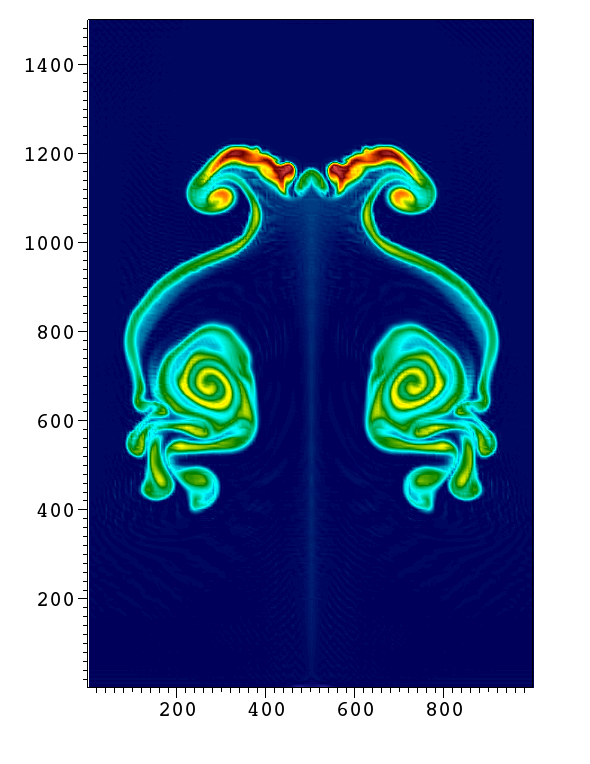
\includegraphics[width=\textwidth]{figures/RTB-Robert--smgo-5mX5m-1080s0000.png}
\caption{2D rising thermal bubble (Robert, 1993) stabilized via a constant coefficient Smagorinsky-Lilly SGS: Potential temperature, $\theta$, at $t=1080\,{\rm s}$. Grid resolution: $\Delta x = \Delta z = 5\,{\rm m}$.}
\label{fig:benchmarks/robert5msmago}
\end{figure}

\subsection{2D density current}
This test is described in \cite{strakaWilhelmson1993}. It consists of a flow that is triggered by the cold perturbation of a neutrally stratified atmosphere at initially uniform potential temperature $\theta_0 = 300$ K
and in hydrostatic equilibrium such that the pressure decreases with $z$ as:
\begin{equation}
\label{pressureDistrib2}
p = p_{0}\left(1-\frac{g}{c_p{\theta_{0}}}z\right)^{c_p/R}.
\end{equation}
The domain $\Omega=[-25600,25600]\times[0,6400]\,{\rm m}^2$.
The perturbation is linear and defined as
\begin{equation}
 \Delta\theta = \left\{ \begin{array}{ll}
 0 & \mathrm{if } r > 1\,{\mathrm K}\\
 0.5 \theta_c \left(1 + \cos(\pi r) \right) \leq 1\,{\mathrm K}\\
\end{array} \right.
\label{eq:robertIni2}
\end{equation}
where $r = \sqrt[]{(x-x_{c})^2/r_x^{2} + (z-z_{c})^{2}/r_z^2}$, $(x_c,z_c) = (0,4000)\,{\rm m}$, $(r_x, r_z) = (4000, 2000)\,{\rm m}$ and $\theta_c=-15$ K. The fully developed density current at $t=900\,{\rm s}$ simulated with a grid effective resolution of $25$ m in both spatial directions is shown in Figure \ref{fig:benchmarks/dc25msmago}.

\begin{figure}[htbp]
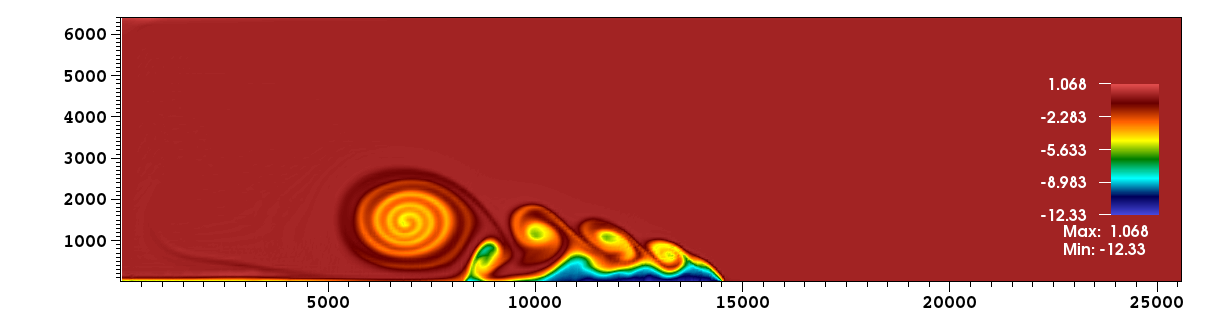
\includegraphics[width=1.2\textwidth]{figures/DC-smgo-25mx25m-900s0000.png}
\caption{2D density current stabilized via a constant coefficient Smagorinsky-Lilly SGS. Potential temperature, $\theta$, at $t=900\,{\rm s}$ (top) and at $t=1200\,{\rm s}$ (bottom). Grid resolution: $\Delta x = \Delta z = 25\,{\rm m}$.
}
\label{fig:benchmarks/dc25msmago}
\end{figure}


%%
\subsection{Rising thermal bubble in a saturated atmosphere}
\label{rtb3D}
The moist dynamics is tested by means of the saturated rising bubble test described in \cite{Pressel15a}. The initial conditions are setup as follows:

\begin{itemize}
\item Initialize dry atmosphere with uniform background $\theta_{ref} = 320$ K
\item Add thermal perturbation $\Delta \theta$ of radius $r=2$ km
\item Set a uniform total mixing ratio $q_t = 0.0192 \,{\rm kg/kg}$ and $q_l = q_i = 0.0\,{\rm kg/kg}$
\item Calculate the gas constants for moist air: 
\[\begin{array}{lcl}
R_{gas} &=& {\tt MoistThermodynamics.gas\_constant\_air(q_t, q_l, q_i)}\\
c_v     &=& {\tt MoistThermodynamics.cv\_m(q_t, q_l, q_i)}\\
c_p     &=& {\tt MoistThermodynamics.cp\_m(q_t, q_l, q_i)}\\
\end{array}
\]
\item  Compute $\theta$, $\rho$, and $T$ as if the background were dry:\\
    \[ \begin{array}{lcl}
  \theta &=& \theta_{ref} + \Delta\theta\\
 \pi & =& 1 - gz/(c_p\theta)\\
 \rho & = & p_0/(R_{gas}\theta)\pi^{c_v/R_{gas}}\\
 T   & = &\pi \theta
\end{array}\]

\item Add the contribution of moisture to the internal energy and recalculate $T$ and $P$, and obtain $e^{\rm tot}$ using the following {\tt MoistThermodynamics} functions:
\[\begin{array}{lcl}
I &=& {\tt MoistThermodynamics.internal\_energy(T + T_0, q_t, q_l, q_i)}\\
T &=& {\tt MoistThermodynamics.air\_temperature(I, q_t, q_l, q_i)}\\
P &=& {\tt MoistThermodynamics.air\_pressure(T - T_{ref} , \rho, q_t, q_l, q_i)}\\
e^{\rm tot} &=& {\tt MoistThermodynamics.total\_energy(0.5\|{\bf u} \|^2, gz, T, q_t)}
\end{array}\]
\end{itemize}

%%
\subsection{Dynamics and Chemistry of Marine Stratocumulus: DYCOMS RF01}

\cite{Stevens05a} provide the following initial distribution of liquid water potential temperature,
\begin{equation}\label{eq:dycoms1}
\theta_l(z) = 
    \begin{cases}
    289.0\;\mathrm{K} & z\leq z_i,\\
    297.5 + (z - z_i)^{1/3}\;\mathrm{K}& z > z_i,
    \end{cases}
\end{equation}
and total specific humidity, 
\begin{equation}\label{eq:dycoms2}
q_t(z) = 
    \begin{cases}
    q_{t,0} & z\leq z_i,\\
    1.5\;\mathrm{g/kg} & z > z_i.
    \end{cases}
\end{equation}
Here, $z_i$ is the initial cloud top set to $z_i=840\,{\rm m}$. \cite{Stevens05a} state that ``modeling groups were also asked to standardize their thermodynamic calculations'' so that the initial state corresponds to a cloud layer between 600 and 800~m with liquid water specific humidity
\begin{equation}\label{eq:dycoms2}
q_l(z) = 
    \begin{cases}
    0 & z\leq 600~\mathrm{m},\\
    0.45\frac{{}z - 600~\mathrm{m}}{z_i - 600~\mathrm{m}}\;\mathrm{\frac{g}{kg}}   & 600~\mathrm{m} < z \leq z_i,\\
    0 & z > z_i.\\
    \end{cases}
\end{equation}
With our thermodynamics and standard thermodynamical constants, we obtain such a cloud layer if we choose the initial total specific humidity in the mixed layer to be $q_{t,0} = 8.1\;\mathrm{g/kg}$, which is slightly lower than the DYCOMS default value of $9\;\mathrm{g/kg}$.

To specify the thermodynamic state completely, we additionally need to specify an initial density. We do so by first specifying an initial pressure
\[
p_0(z) = p_{s} \exp(-z/H), \qquad H = \frac{R_m T_0}{g},
\]
where $R_m = R_m(q_t, q_l)$ is the gas constant for moist air, $T_0 = 285.0~\mathrm{K}$ is an average boundary-layer temperature, and $p_s = 1.0178\times 10^{5}~\mathrm{Pa}$ is the surface pressure, with surface density $\rho_s = 1.22~\mathrm{kg/m^3}$ and surface temperature $T_s = p_s/(\rho_s R_{m,s})$. Consistent with the Boussinesq or anelastic approximation used in most DYCOMS simulations, we calculate thermodynamic quantities with this reference pressure $p_0(z)$. We use the linearized expression for the liquid-water potential temperature,
\begin{equation}
    \label{eq:betts1973}
    \theta_l = \theta \left(1 - \frac{L_{v,0} q_l}{c_{pm} T} \right) = \theta - \frac{L_{v,0} q_l}{c_{pm} \Pi_0},
\end{equation}
where $\theta = T/\Pi_0$, and 
\[
\Pi_0 = \left( \frac{p_0(z)}{p_{s}} \right)^{R_d/c_{pd}}
\]
is evaluated with the pressure profile $p_0(z)$. This can be solved for temperature as a function of height $z$,
\[
T = \Pi_0 \theta_l + \frac{L_{v,0} q_l}{c_{pm} \Pi_0},
\]
given $\theta_l(z)$, $q_l(z)$, and $\Pi(z)$. Density is then obtained from the ideal gas law as
\[
\rho(z) \approx \frac{p_0(z)}{R_m T(z)},
\]
thus completely specifying the initial state. 

The initial state of all the quantities described above are plotted in Figure \ref{dycomsInitFig}
\begin{figure}
    \centering
	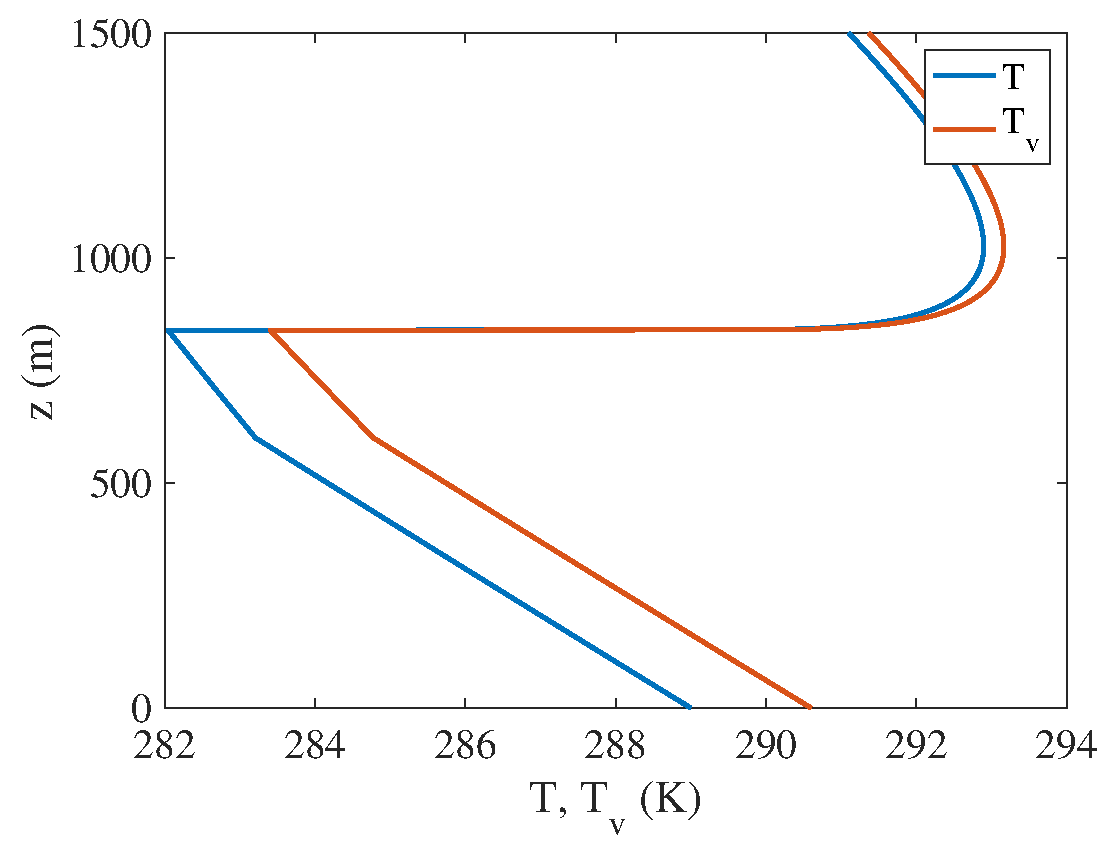
\includegraphics[width=0.49\textwidth]{./figures/dy_tempe.eps}
	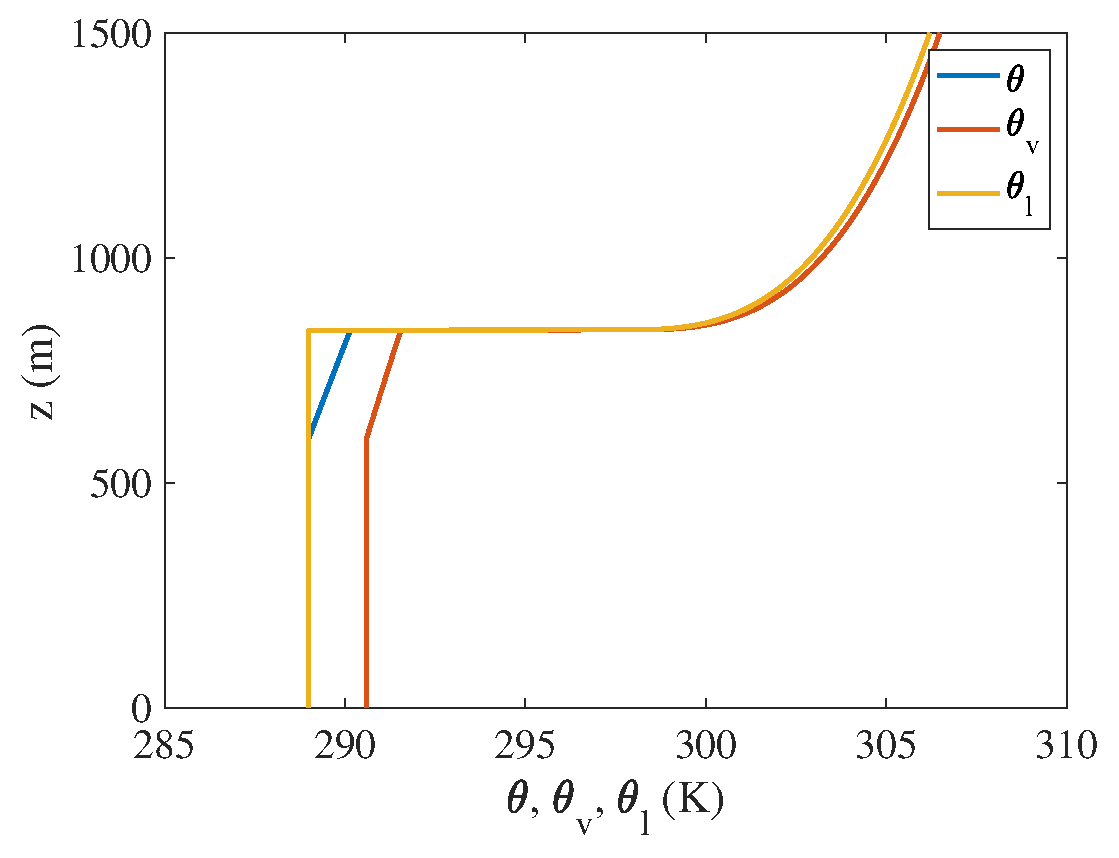
\includegraphics[width=0.49\textwidth]{./figures/dy_pot_temp.eps}
	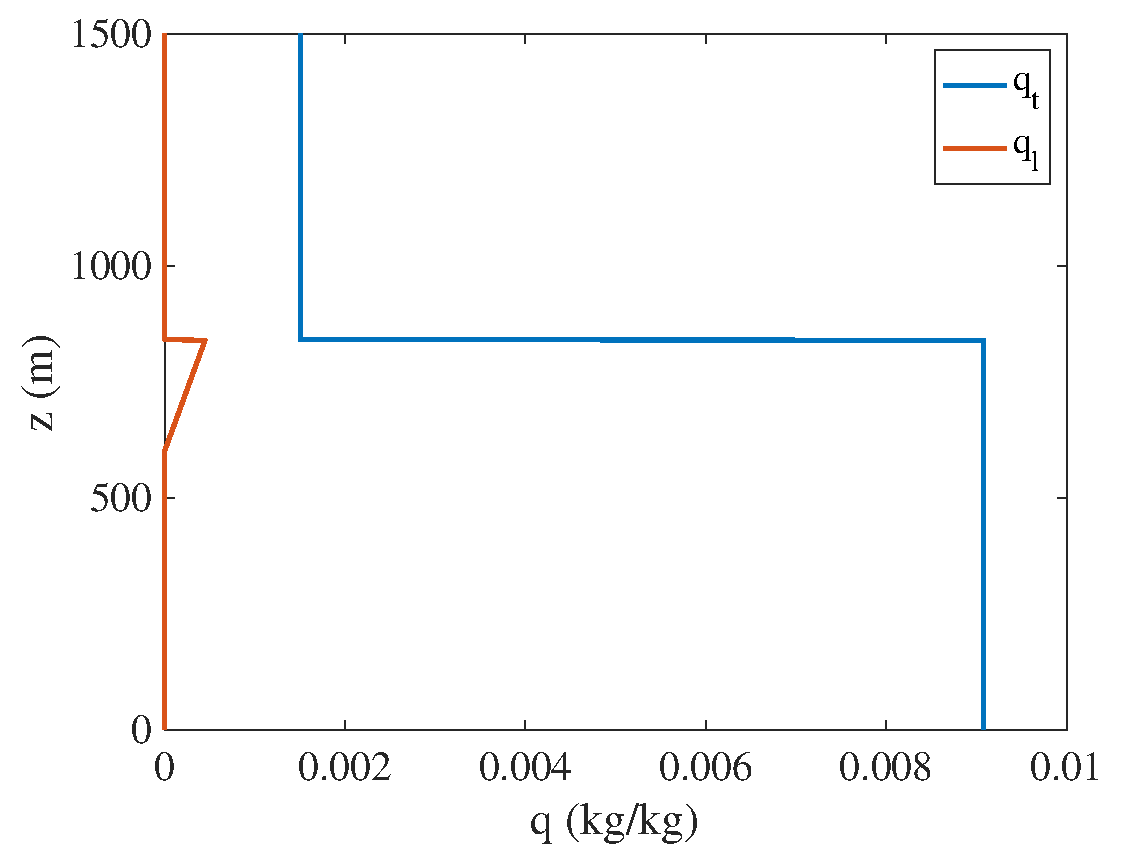
\includegraphics[width=0.49\textwidth]{./figures/dy_mixing_ratios.eps}
	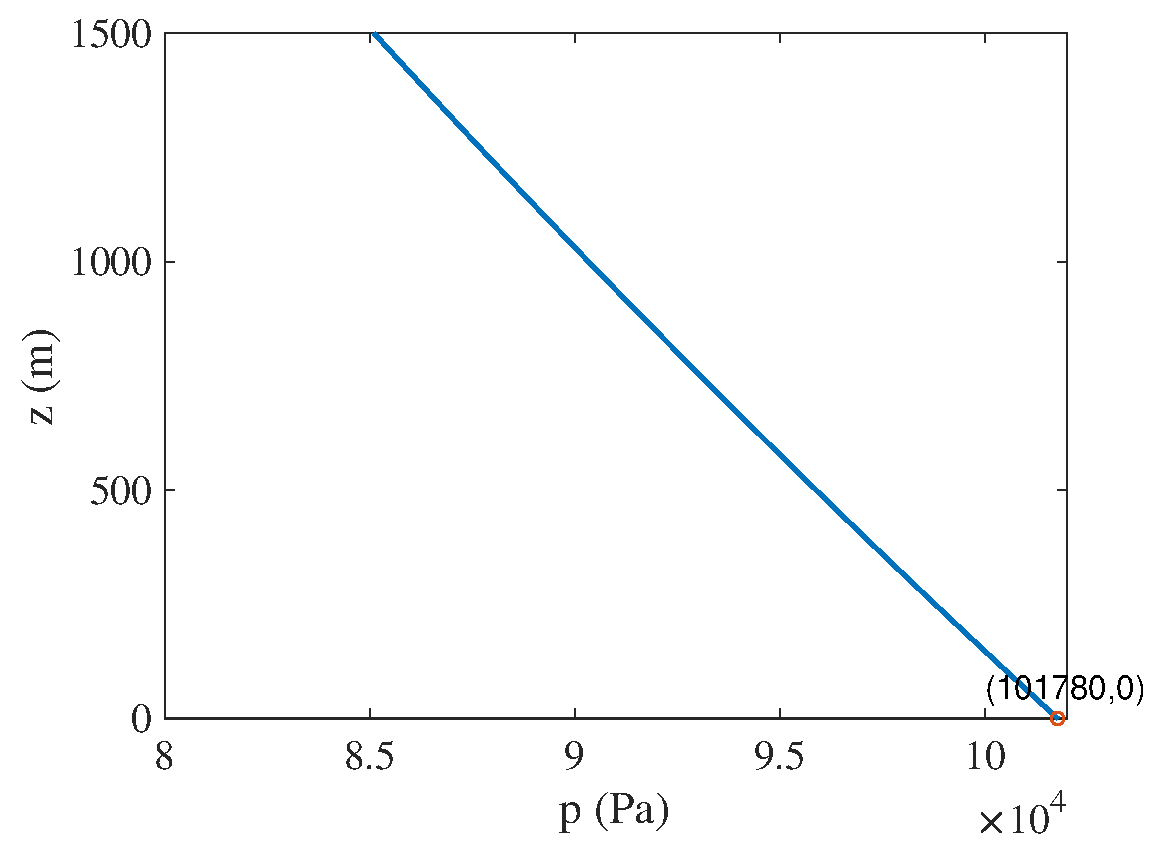
\includegraphics[width=0.49\textwidth]{./figures/dy_press.eps}
	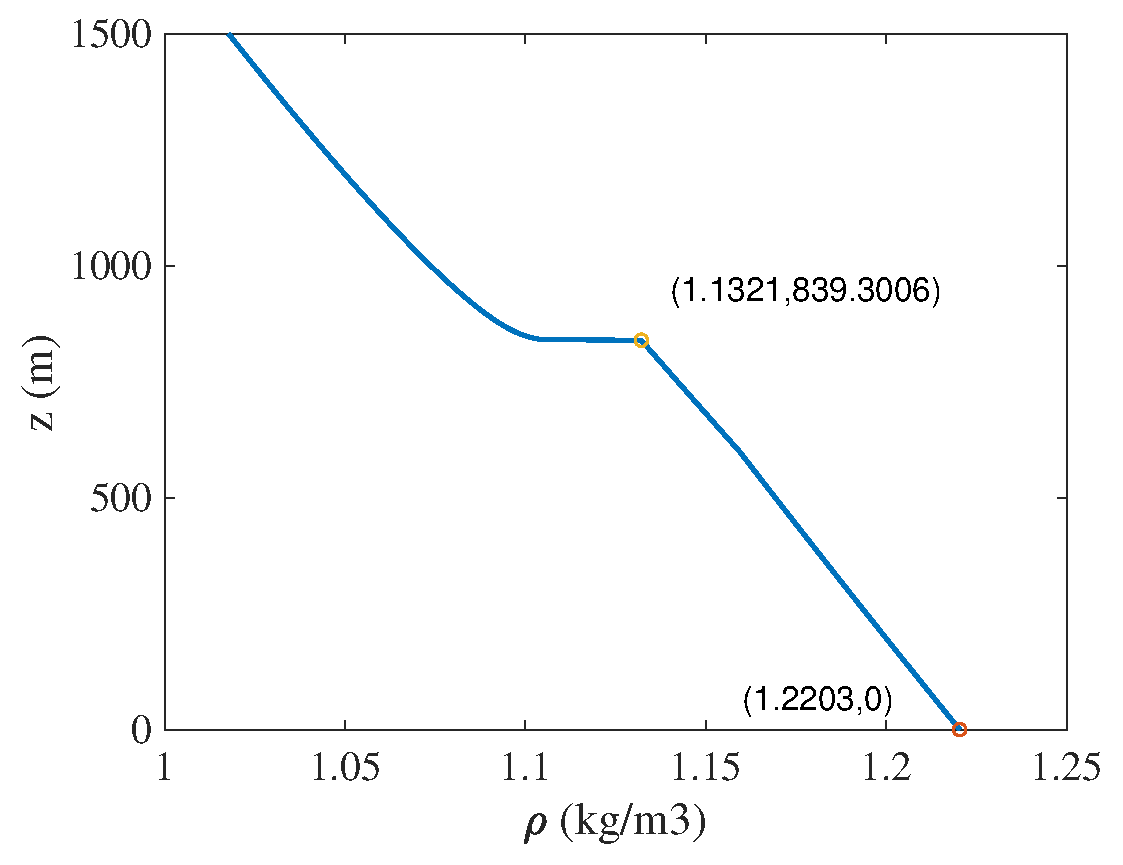
\includegraphics[width=0.49\textwidth]{./figures/dy_densi.eps}
	%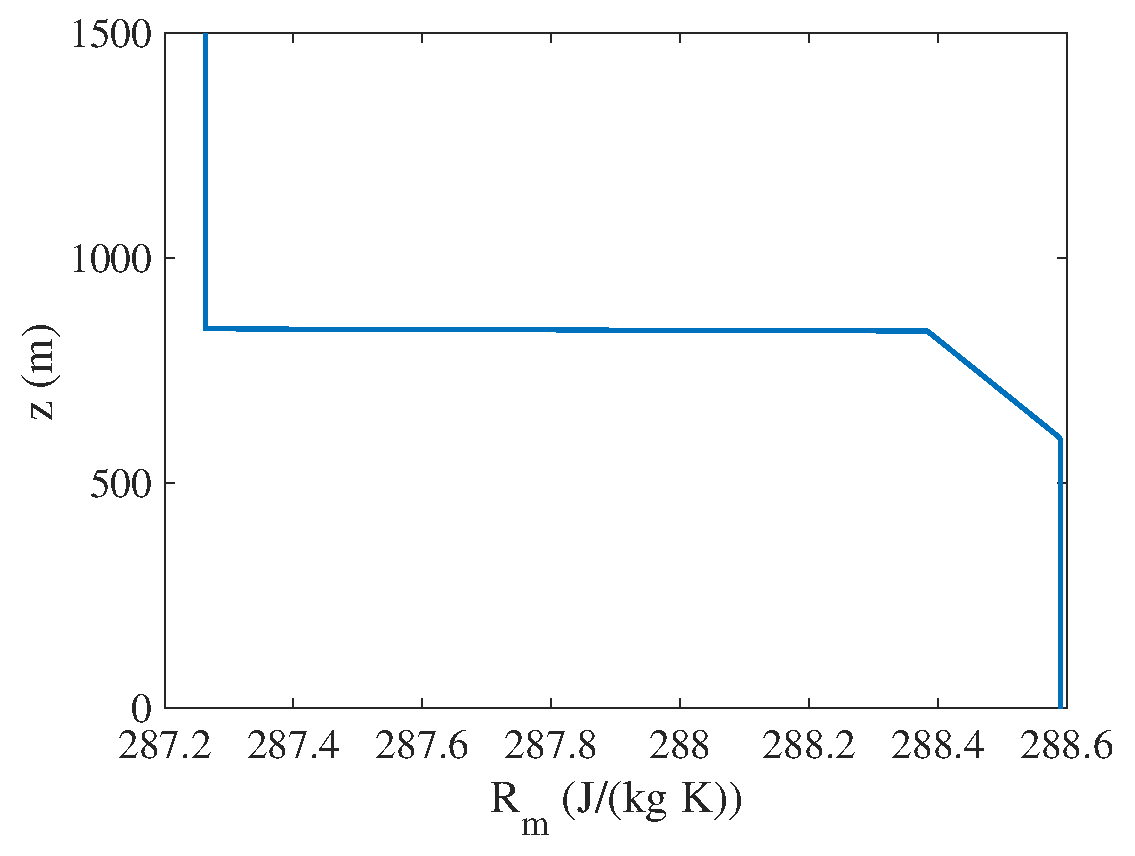
\includegraphics[width=0.49\textwidth]{./figures/dy_Rm.eps}
	%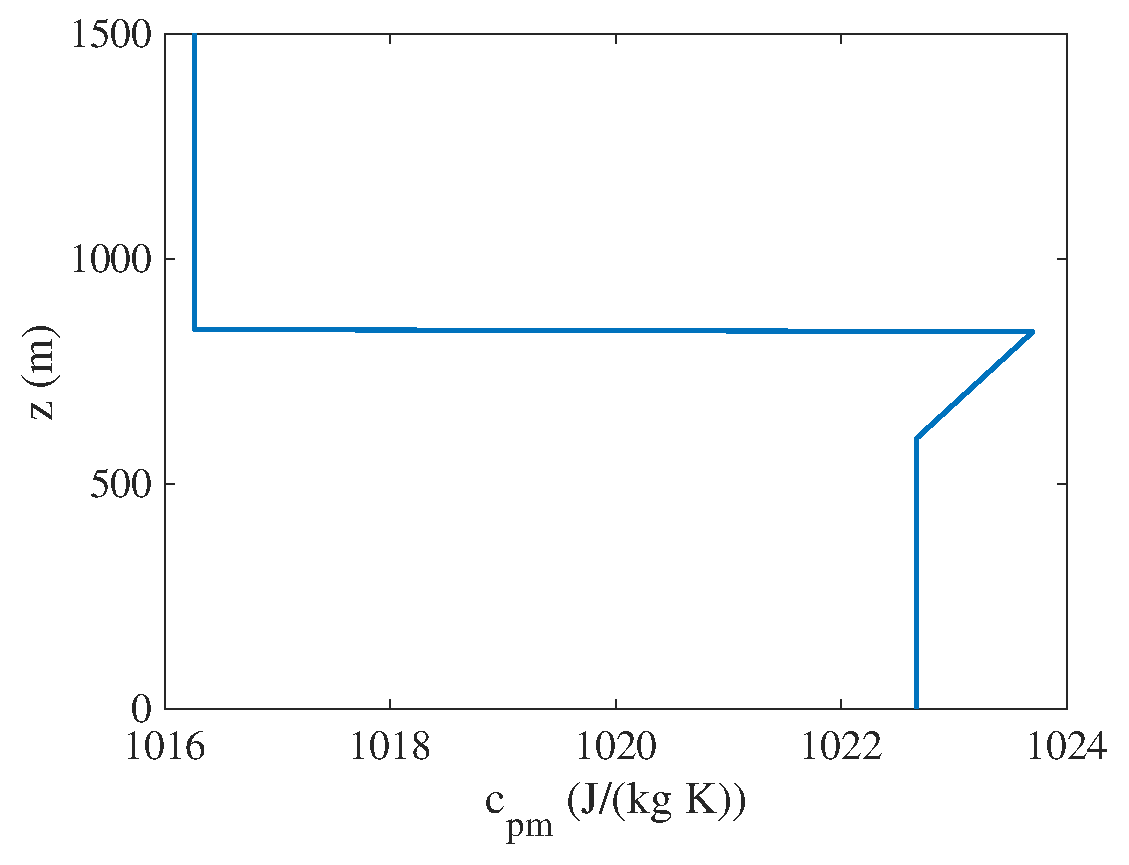
\includegraphics[width=0.49\textwidth]{./figures/dy_cpm.eps}
      \caption{Dycoms: initial states of $T, T_v, \theta, \theta_v, \theta_l, q_t, q_l, p, \rho$.}
\label{dycomsInitFig}
\end{figure}

\hl{[Specify forcing functions, e.g., radiation, surface fluxes]}
\paragraph{Forcing functions and boundary conditions:}

Bottom boundary conditions should be applied according to \S \ref{s:bottom_bc}. For the time being, in first approximation we are applying the following forcing instead:

\begin{itemize}
    \item Weakly imposed Dirichlet on bottom temperature: $T=SST=292.5\,{\rm K}$.\\
    \item Weakly imposed Dirichlet on bottom $q_t$: $q_t=13.84e-3\,{\rm kg/kg}$.\\
    \item Weakly imposed no-slip: ${\bf u}= 0$.\\
    \item Weakly imposed $SHF = 15\,{\rm W/m^2}$ and $LHF = 115\,{\rm W/m^2}$.\\
\end{itemize}

\paragraph{Radiative cooling}
Radiative cooling is imposed by means of the simple model described by \cite{Stevens05a} which is added to the non-viscous flux of the energy equation. this radiative flux, based on the $\delta$-four stream model \citep{fuLiu1993} is given as the column-wise integral:

\begin{equation}
    \label{e:radiativeStevens05}
    F_{rad}({\bf x}, t} = F_0{\rm e}^{-Q(z,\infty)} +
    F_1\exp\left(-Q(0, z)\right) +
    \rho_i\,c_p\,D\,\alpha_z\[\frac{(z-z_i)^{4/3}}{4} + z_i(z - z_i)^{1/3} \],
\end{equation}
where 
\begin{equation}
    Q(a,b) = \kappa\int_{a}^{b}\rho\,q_l\,dz.
\end{equation}
The following parameters are used:
$F_0=70\,{\rm W\,m^{-2}}$, $F_1=22\,{\rm W\,m^{-2}}$, $\kappa=85\,{\rm m^2\,kg^{-1}}$, $\alpha_z=1\,{\rm m^{-4/3}}$. The large scale subsidence divergence is parameterized by $D=3.75\time 10^{-6}\,{\rm s^{-1}}$. This value is also used to calculate the subsidence velocity as $w=-Dz$.


\subsection{3D squall line}
\label{sq3D}
The three-dimensional simulation of a squall line is defined in the domain 
$80\times 80\times20\,{\rm km}^3$. 
The initial background state is given by the sounding of \cite{gabersekGiraldoDoyle2012}.
To initiate the vertical transport of water vapor to a level of condensation (and hence trigger a cloud formation, the initial background is forced by a temperature anomaly $\theta'$ $3$ K warmer than the surrounding environment. 

A stretched grid along $z$ is used to make the resolution higher in the lower atmosphere where convection is triggered.
The domain is crossed by a horizontal wind along the x-direction with a $12\,{\rm m\,s^{-1}}$ shear at $z=2000\,{\rm m}$.
A no-slip condition is applied on the surface boundary while periodic boundaries are defined along $x$ and $y$. 
To damp the vertically propagating gravity ways triggered by the cloud formation, a Rayleigh absorbing layer is applied at the higher layers of the atmosphere.
The cloud first forms at approximately 500 s, and is fully develop after 4500 s. 
An instantaneous view of the precipitating squall line is shown in Figure \ref{fig:benchmarks/squall1}. 

\begin{figure}[htbp]
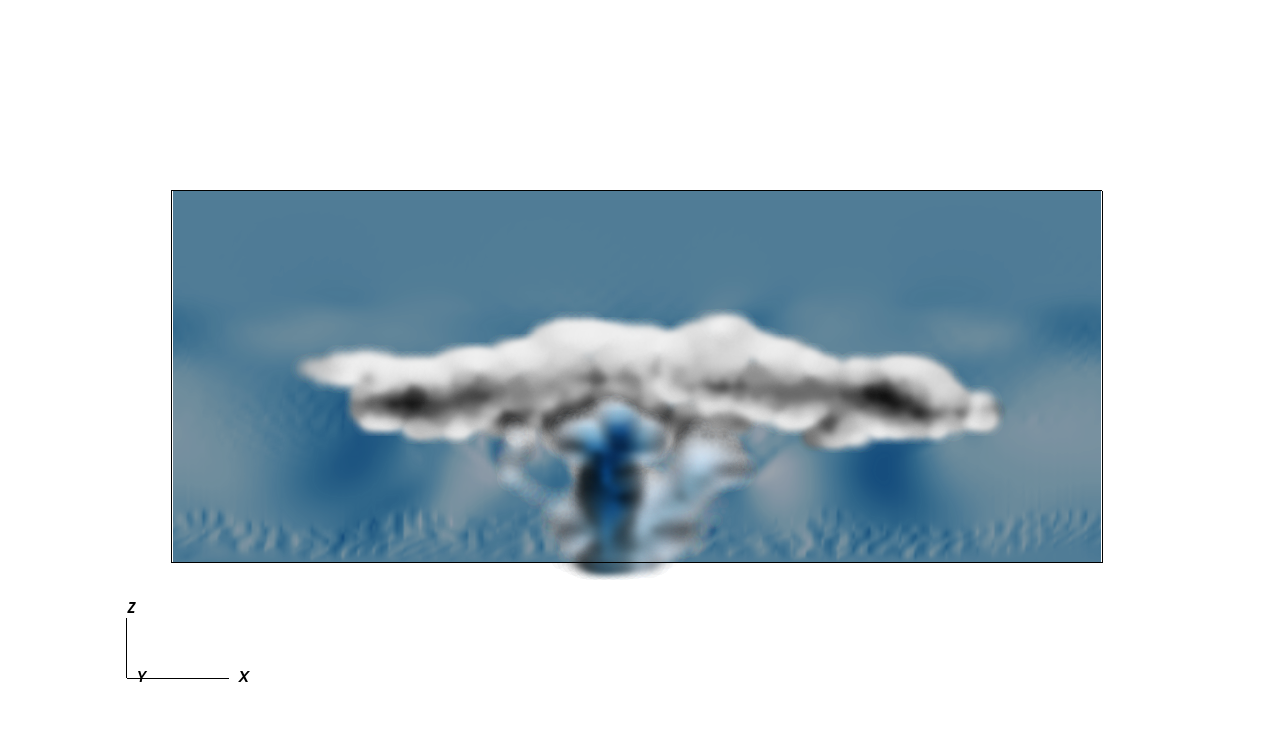
\includegraphics[width=1.2\textwidth]{figures/squall_working_warm_rain_frontal_view0028.png}
\caption{Front view of a fully developed squall line with precipitating rain. }
\label{fig:benchmarks/squall1}
\end{figure}


\subsection{External soundings}
External soundings can be read into the code for initialization purposes. The sounding requires the format reported in Table \ref{tab:DeltaDefinitionsTable}.

\begin{table*}[t]
\centering
{\footnotesize
\caption[short]{Structure of sounding files for simulation initialization.}
\label{tab:DeltaDefinitionsTable}
\begin{tabular*}{\textwidth}{ @{\extracolsep{\fill}} llllll}
\hline
\hline
z (m) & $\theta_v$ (K) & $q_{tot}$ $\rm {kg/kg}$ & $u$ (m/s) & $v$ (m/s) & p (Pa)\\
0 & 300 & 14  & -2 & 0 & 100000\\
... & ... & ...  & ... & ... & ...\\
\hline

\hline
\hline
\end{tabular*}
}
\end{table*}

\subsection{Held-Suarez GCM benchmark}

%-------Bibliography
\bibliographystyle{agufull08}
\bibliography{Giraldo_refs,CLIMA-refs}

\end{document}
